%----------------------------------------------------------------------------
\chapter{User Documentation}\label{ch:user}
%----------------------------------------------------------------------------

This chapter walks through the portal page by page from the perspective of someone who has just opened it for the first time. Each section describes the page itself, what is interactive on it, what happens when each part is clicked, and which data file controls what the page shows. The second part is what makes this chapter useful to two different audiences at once: a visitor reading from top to bottom learns how the portal behaves, and a lab member who wants to update something can jump to the relevant page and find the file they need to edit.

The screenshots in this chapter were taken in dark mode. Light mode is available through the toggle on the right side of the header and the layout is identical in both, so the screenshots are not duplicated for each theme.

%-----------------------------------------------------------
\section{Shared Layout}\label{sec:user-shared}

Every page on the portal shares the same header, navigation bar, and footer. These three pieces are part of the layout and appear regardless of which page is currently selected.

\subsection{Header}\label{subsec:user-header}

The header sits at the top of every page. On the left is the ELTE Faculty of Informatics logo. In the centre is the portal title, \textbf{Cybersecurity-Lab}, written in a decoded-text effect: on the first load it looks like a scrambled string and then resolves into the readable title. Both the logo and the title are clickable and both return the visitor to the home page no matter where they are. On the right is a sun-and-moon icon that toggles the entire portal between light and dark mode in place, without a page reload.

The development banner on the top-left corner (``UNDER DEV'') is currently shown to signal that the portal is still being worked on. It is controlled by a flag in the site configuration and will be removed when the lab decides the portal is ready to be considered live.

\subsection{Navigation Bar}\label{subsec:user-nav}

Below the header is the navigation bar with eight items: \textbf{Projects}, \textbf{Research}, \textbf{Operations}, \textbf{CodeBases}, \textbf{Publications}, \textbf{Team}, \textbf{Mini Apps}, and \textbf{Gallery}. Each item routes to the corresponding page and the currently active page is highlighted with a filled background. The order of the items follows the natural reading order of the portal: research direction first, then operational structure, then the artefacts (codebases, publications), then the people, then the interactive tools and visual content.

\paragraph{Data file.} The contents of the navigation bar live in \texttt{src/data/navigationItems.ts}. Each entry has a \texttt{label} (the text shown in the bar) and a \texttt{path} (the route the link goes to). Reordering entries in this file reorders the navigation bar. Renaming a label changes the displayed text. The \texttt{path} should not be changed because it is matched against the React Router configuration; changing it would orphan the route. New navigation items can be added by adding a new entry, but adding an entry without a matching route in the application will produce a broken link.

\subsection{Footer}\label{subsec:user-footer}

The footer sits at the bottom of every page and contains the lab's identity information: the ELTE Faculty of Informatics logo on the left, the lab name and department in the centre, the address, the university and faculty links, and on the right two buttons, \textbf{Contact} and \textbf{GitHub}. The Contact button opens the Contact page. The GitHub button opens the lab's GitHub organisation in a new tab.

\paragraph{Data file.} The footer content is driven by \texttt{src/data/siteConfig.ts}. This file holds the lab's short name, the university, the faculty, the department, the address (street, city, postal code, country), and the external links (GitHub organisation, university homepage, faculty homepage). Changes to any of these fields propagate to the footer on every page.

%-----------------------------------------------------------
\section{Home Page}\label{sec:user-home}

The home page is what a first-time visitor sees when they open the portal. It is the only page where no navigation item is highlighted in the bar. At the top of the content area sits a short introduction describing the lab in a single sentence. Below it is an interactive hexagonal grid showing the lab's research areas. Each hex is clickable; clicking one opens a panel below the grid with the full description of that research area.

In the background of the page, a soft animated network of nodes connected by lines runs continuously. The animation is decorative: small particles travel along the lines between nodes, suggesting data flow. The animation pattern changes subtly when the visitor interacts with the hexagonal grid.

Toward the lower part of the page there is a card for the \textbf{Security Gauntlet} mini-app. Clicking the card opens the Security Gauntlet directly without going through the Mini Apps page first. The card is on the home page because the game is the most visually striking interactive piece in the portal and serves as a way of pulling first-time visitors into the interactive content.
\begin{figure}[H]
	\centering
	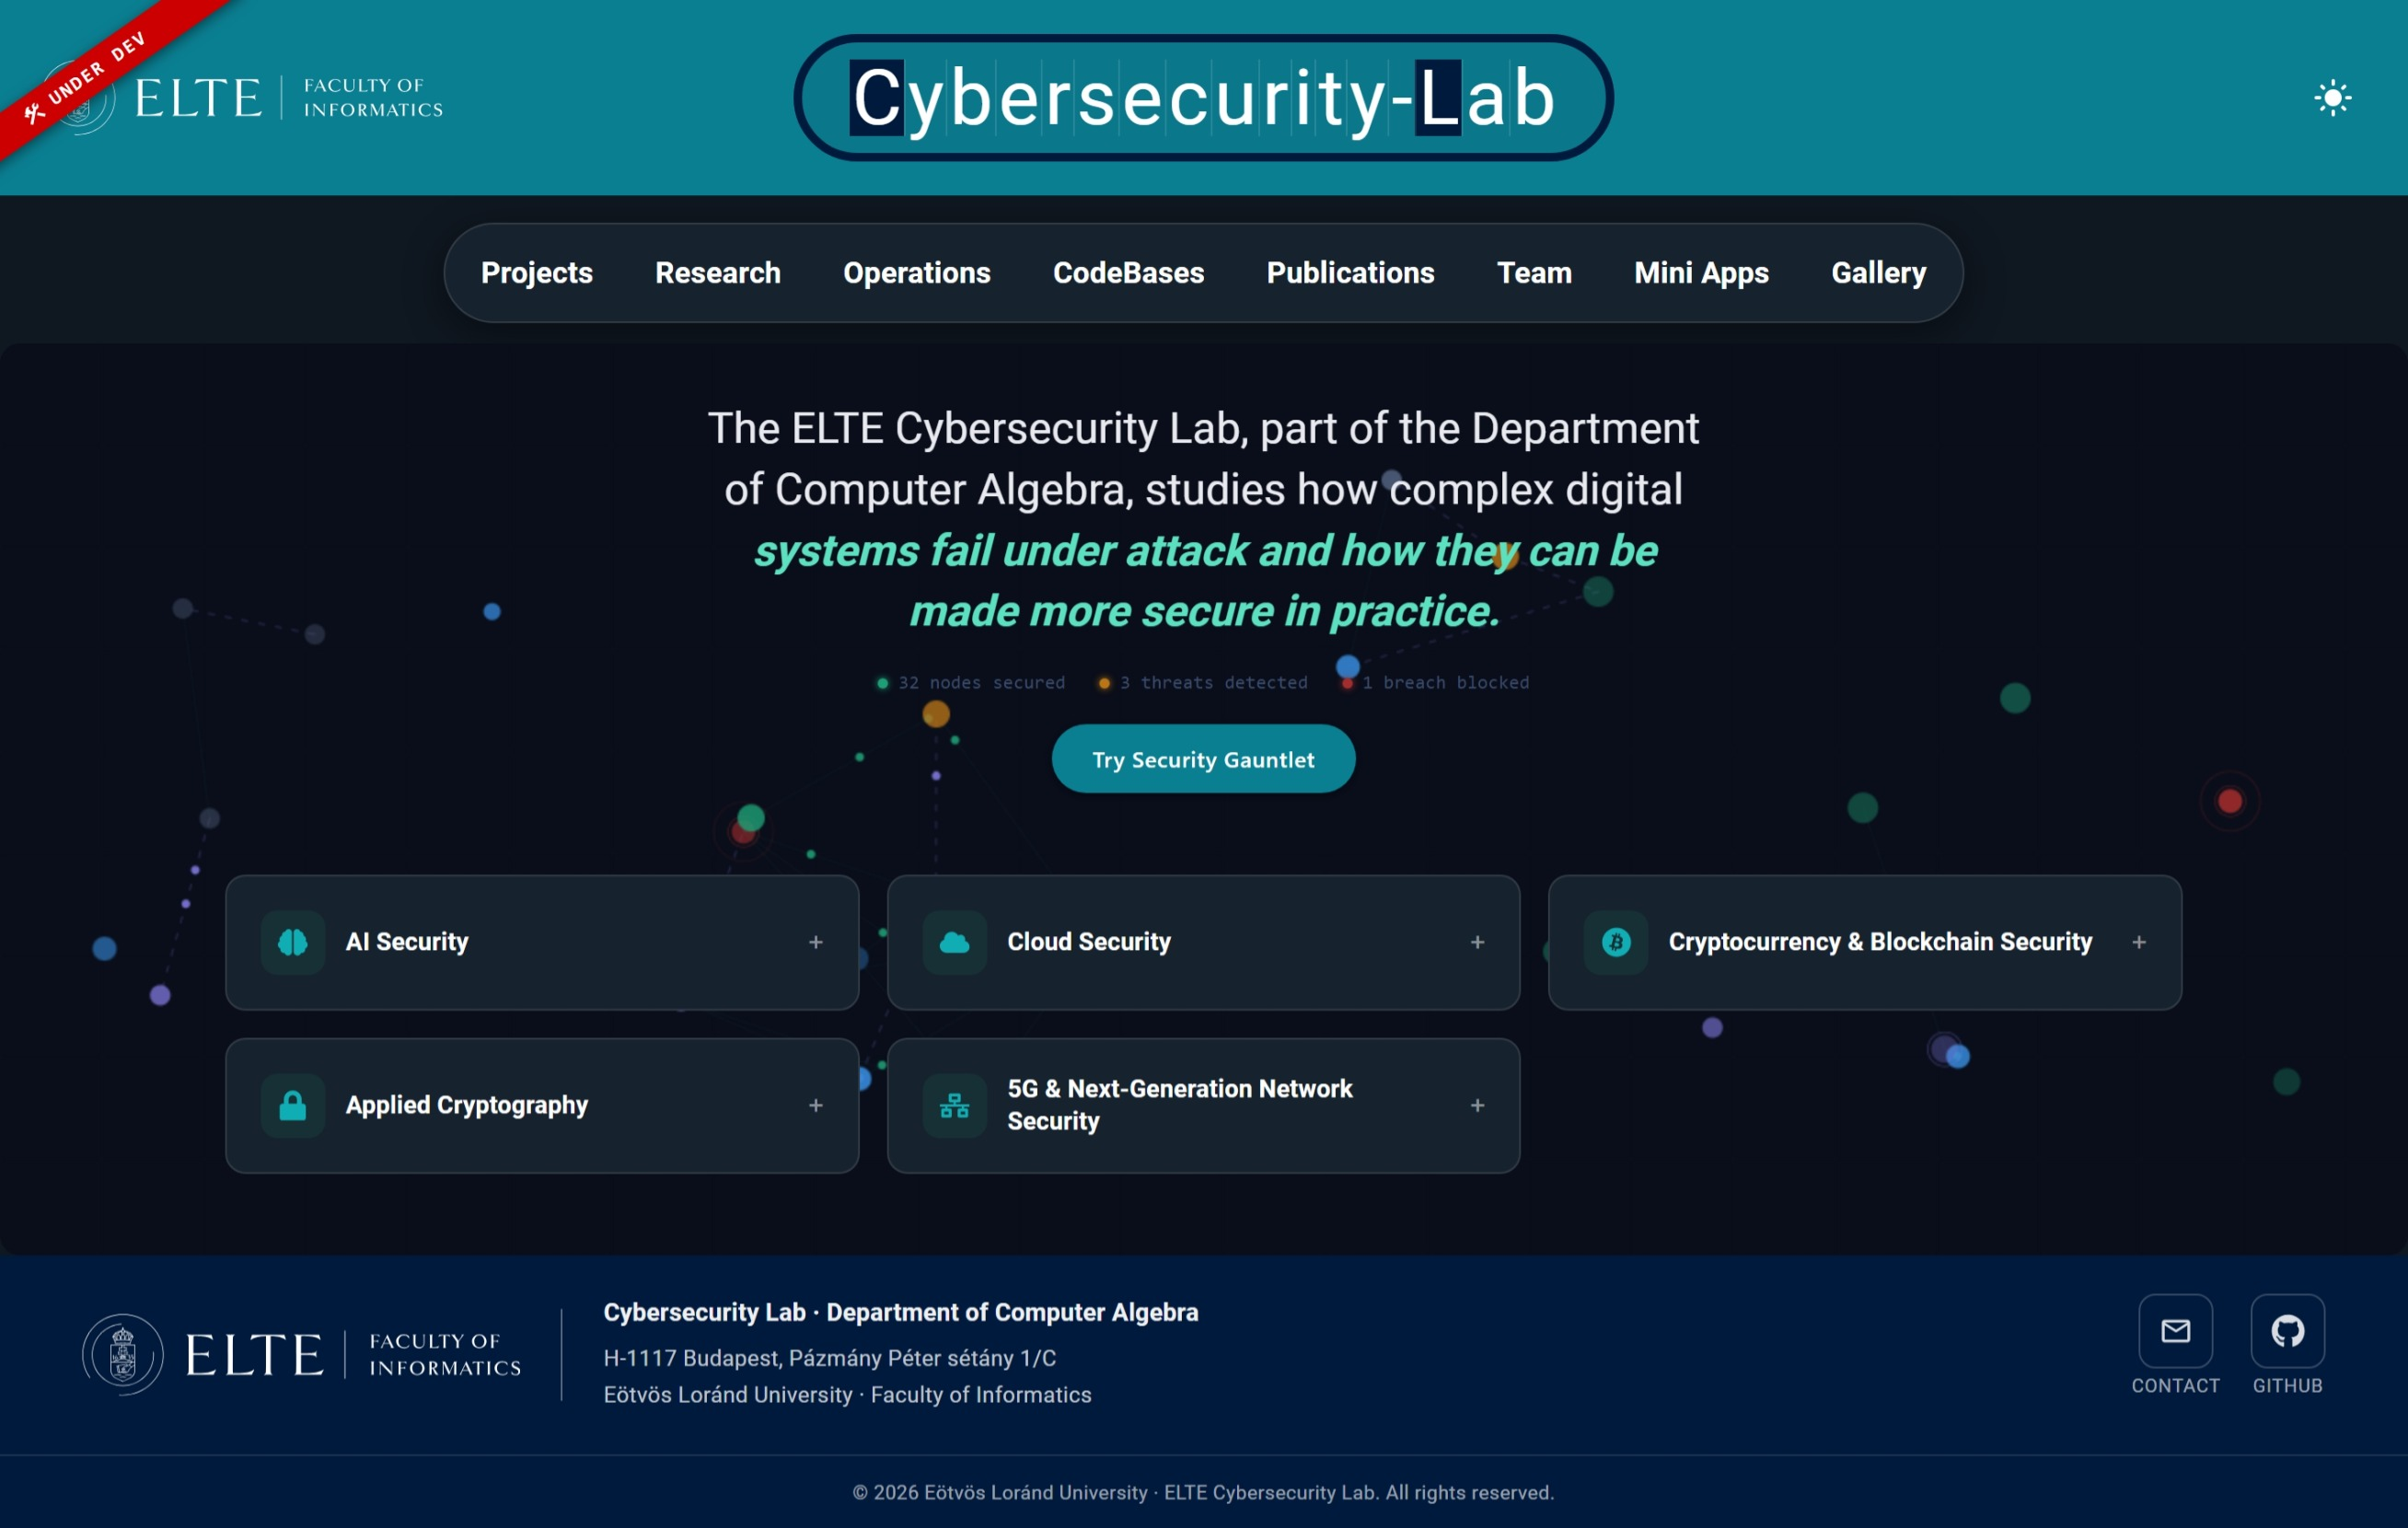
\includegraphics[width=0.88\textwidth]{images/home.jpeg}
	\caption{The Home page with the animated node background, the hexagonal research grid, and the Security Gauntlet card lower down.}
	\label{fig:home}
\end{figure}

\paragraph{Data file.} The text shown on the home page and the list of research areas it displays come from \texttt{src/data/HomePageData.ts}. The file exports \texttt{MainTitle}, a single string used as the lab's headline, and \texttt{researchAreas}, an array of \texttt{\{title, description\}} objects. Editing \texttt{MainTitle} changes the headline. Adding, removing, or editing entries in \texttt{researchAreas} changes the cards under the headline. The file is intentionally lighter than the Research page's data file because the home page shows a simpler summary.

%-----------------------------------------------------------
\section{Projects Page}\label{sec:user-projects}

The Projects page shows the lab's main research projects as a diamond-shaped node graph. There are four outer circles, one per project, and one central circle labelled \textbf{Lab Projects}. The outer circles are colour-coded and labelled with their short names (B5G Network Security, Distributed ML Security, Compliance Verification, Cloud Security).

When the page first loads, the first project in the list is already selected. The selected node is highlighted on the graph and its details appear in the panel on the right of the graph on desktop, and below the graph on mobile. Clicking any other node selects it and updates the panel immediately. The selected panel shows the project's status, the number of sub-projects it has, the number of related projects, a list of keywords, and the names of related projects with which it shares concerns.

Below the graph is the project detail section. It shows the currently selected project's full description, its main objectives (as a bullet list), and its sub-projects. Each sub-project is a collapsible row. Clicking the row expands it to show the sub-project's full description, its focus areas, and any related codebases. Related codebases are shown as clickable links that lead directly to the corresponding CodeBases page entry, so the visitor can move from a project description to the code that supports it without going through the navigation bar.

The number cards at the top of the page (Main Projects, Sub-Projects, Connections) are computed automatically from the data file. They are not edited separately.

\begin{figure}[H]
	\centering
	
\includegraphics[width=0.72\textwidth]{images/projects.jpeg}
	\caption{The Projects page with the diamond-shaped node graph and the detail panel for the first project (B5G Network Security) open below the graph.}
	\label{fig:projects-page}
\end{figure}

\paragraph{Data file.} The Projects page is driven entirely by \texttt{src/data/projectsPageData.ts}. The file exports an object containing a \texttt{projects} array, where each project entry has a \texttt{slug}, \texttt{title}, \texttt{description}, \texttt{mainObjectives} (a list of strings), \texttt{relatedProjects} (a list of project titles), and \texttt{subProjects} (a list of sub-project objects). Each sub-project has a \texttt{title}, \texttt{description}, \texttt{researchFocus} (a list of strings), and \texttt{codebases} (a list of strings matching codebase slugs).

The \texttt{codebases} field on a sub-project is what creates the link from a project to a CodeBases entry. The portal looks up each string in the list against the codebases data and renders a clickable link if a match is found. The match is by slug, so the string in the project file must correspond to the codebase's identifier; a typo here means the link will not appear, but the rest of the project still renders. The \texttt{relatedProjects} field works similarly: it matches against other project titles in the same file.

%-----------------------------------------------------------
\section{Research Page}\label{sec:user-research}

The Research page presents the lab's research areas as a honeycomb of hexagonal cells. There are six outer cells, one per area, arranged around a central decorative cell that shows a stylised chipset motif. Unlike the Projects page, no area is selected when the page first loads. The visitor has to click a hex to open the detail panel below the honeycomb.

Each hex is coloured according to the area's accent colour, has an icon in its centre (a glyph or a small symbol), and has the area's title underneath. The first load animates the hexes into position around the central chipset on a staggered timer, so the honeycomb assembles itself rather than appearing all at once. Long titles such as \textit{Cryptocurrency and Blockchain Security} are wrapped across multiple lines automatically so they fit inside the hex.

Clicking a hex opens a panel below the honeycomb. The panel shows the area's title, a one-sentence intro in italic, and a longer description. The area's accent colour is used for the panel's heading and side border, which links the hex visually to the panel content. Clicking a different hex updates the panel immediately and re-highlights the selected hex on the honeycomb.

\begin{figure}[H]
	\centering
	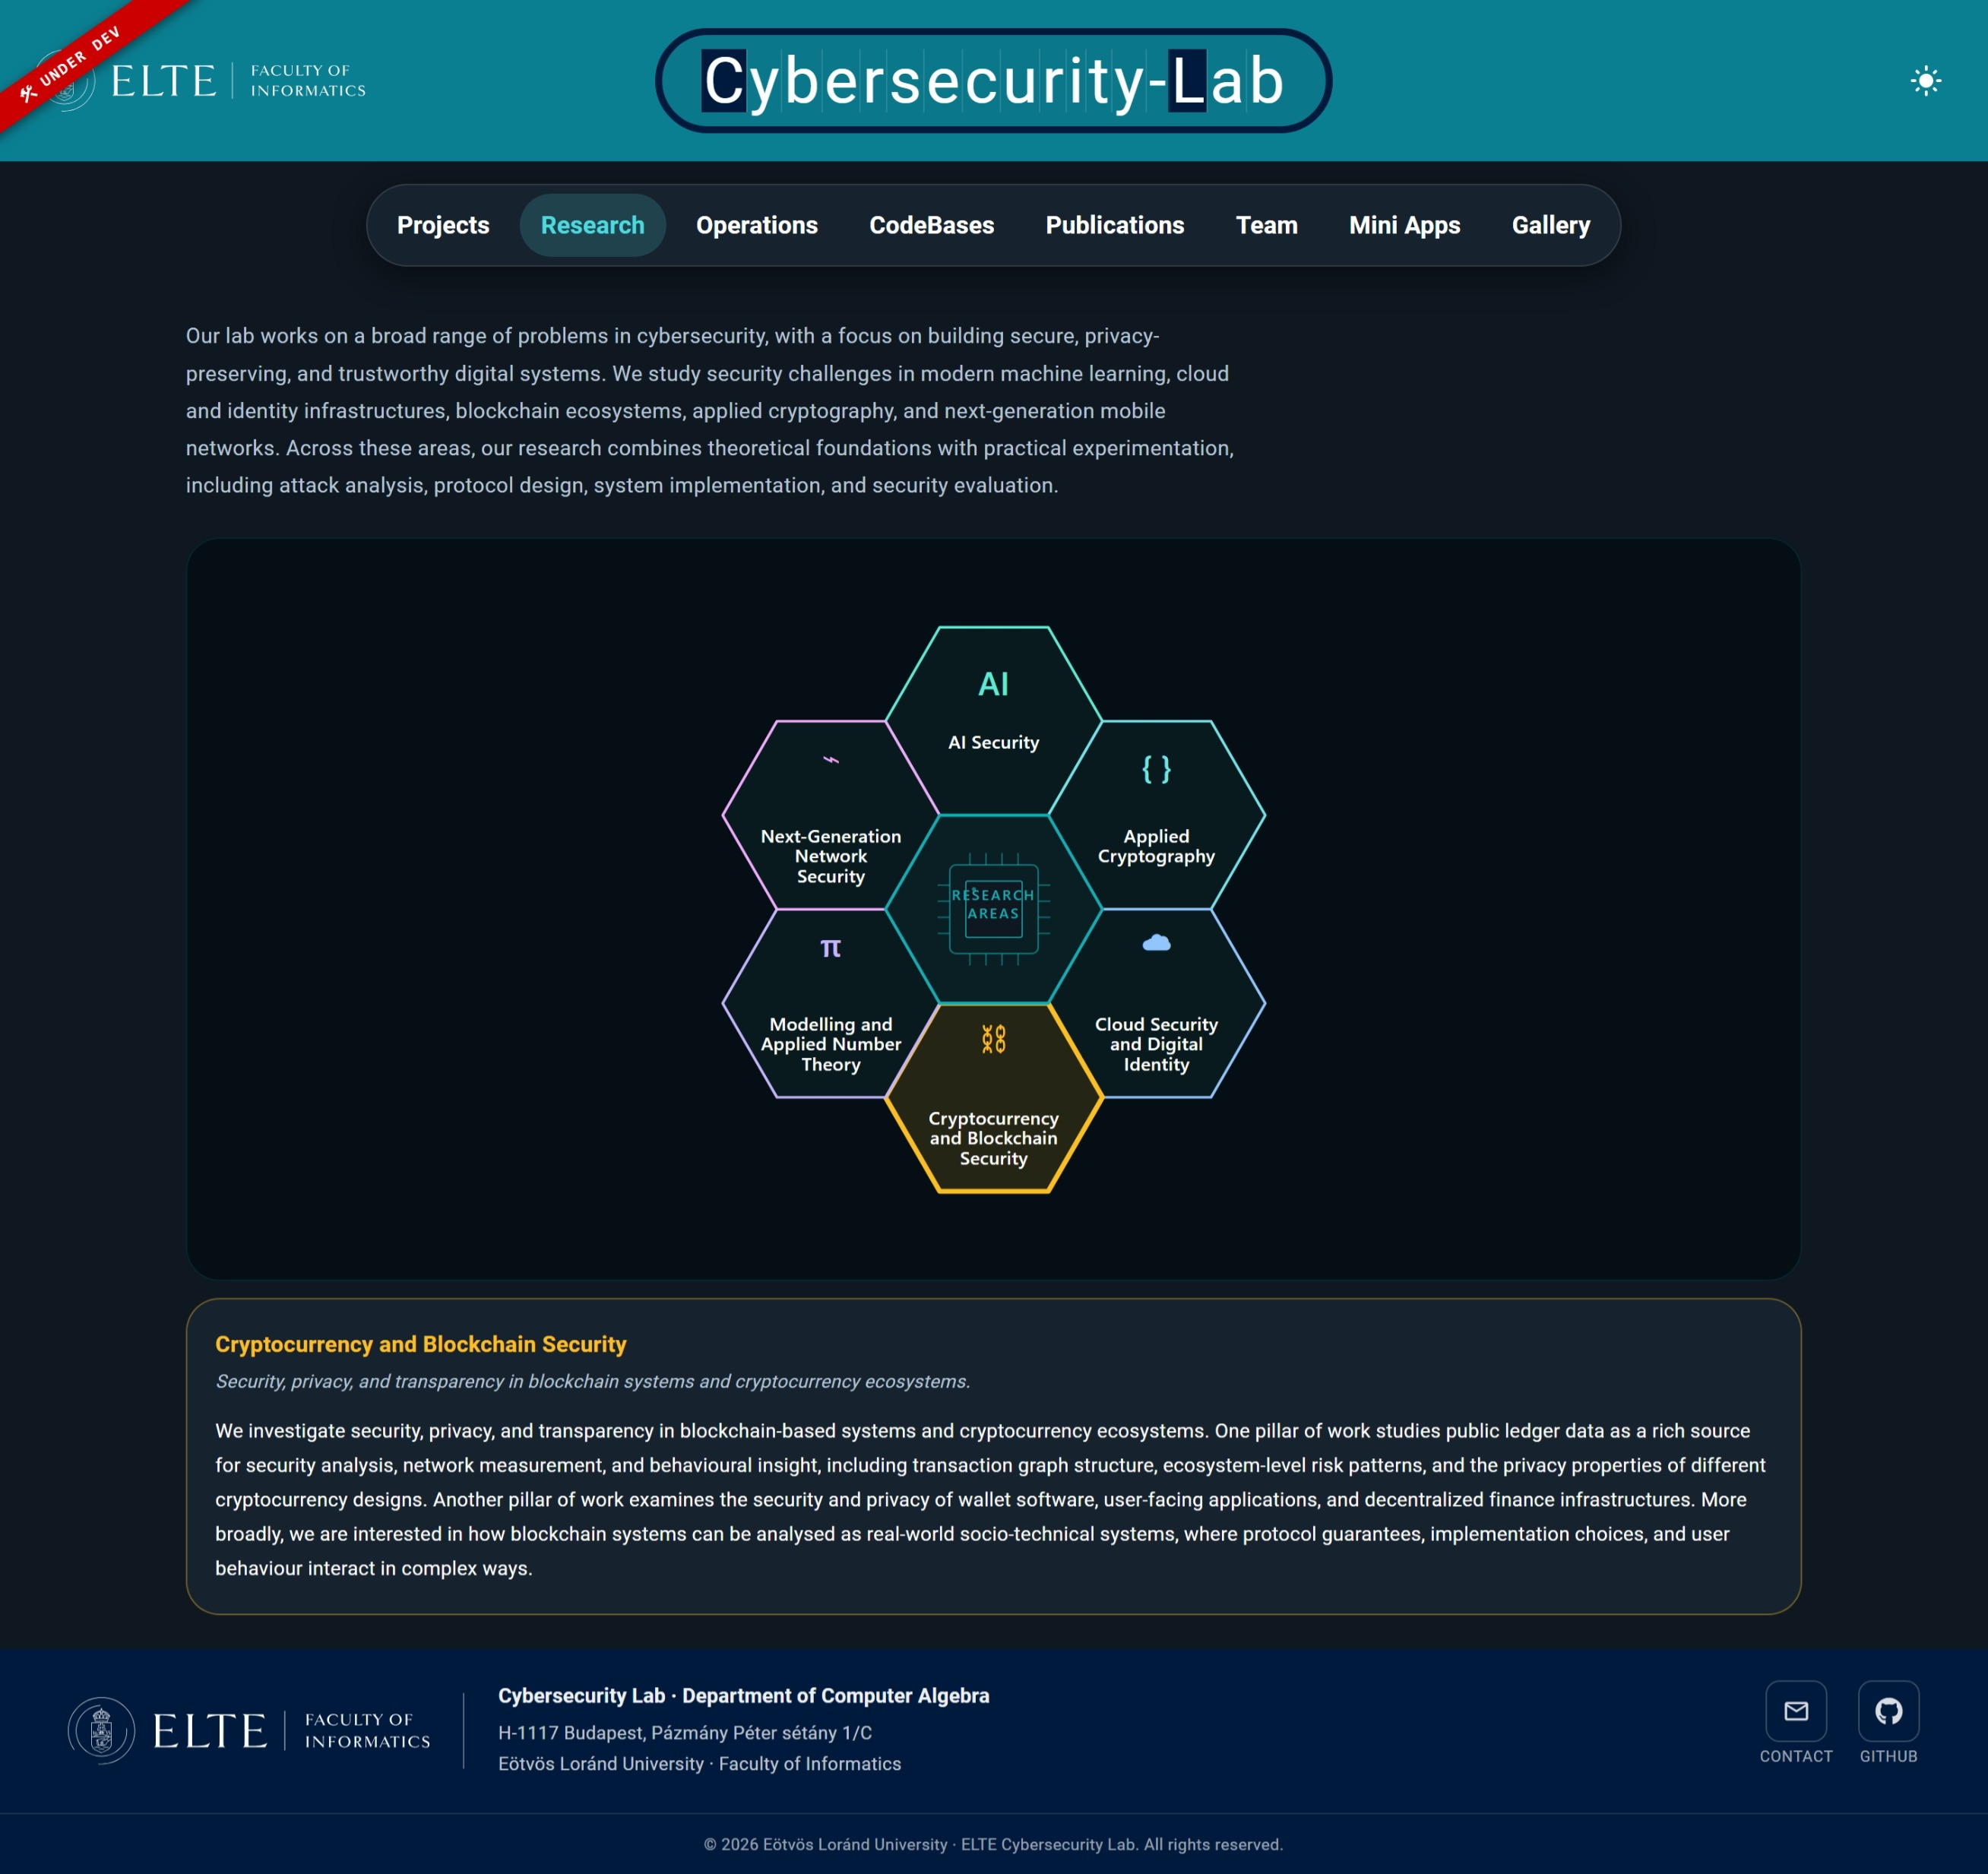
\includegraphics[width=0.88\textwidth]{images/research.jpeg}
	\caption{The Research page with the six-hex honeycomb around the central chipset motif. The Cryptocurrency and Blockchain Security hex is selected and its detail panel is open below the honeycomb.}
	\label{fig:research-page}
\end{figure}

\paragraph{Data file.} The Research page reads from \texttt{src/data/ResearchPageData.ts}. The file exports \texttt{researchPageIntro} (the paragraph shown above the honeycomb) and \texttt{researchAreas} (the array of hex entries). Each research area has an \texttt{id}, \texttt{title}, \texttt{icon}, \texttt{color}, \texttt{intro}, and \texttt{description} field.

The \texttt{color} field accepts any valid CSS colour string and is used for the hex border, the panel heading, and the panel side border. The \texttt{icon} field is a short text glyph rendered inside the hex; using a single character or a couple of characters works best because hexes have limited internal space. Adding a new area requires only a new entry in this array, the honeycomb layout adapts to the number of cells.

%-----------------------------------------------------------
\section{Operations Page}\label{sec:user-operations}

The Operations page describes how the lab organises its work. It opens with a paragraph explaining that lab work is done in small group projects rather than individual assignments. Below the paragraph is the project structure section.

The project structure is shown as a two-by-two grid. The horizontal axis is labelled \textbf{Theory} versus \textbf{Practice}. The vertical axis is labelled \textbf{Builds} versus \textbf{Breaks / Measures}. Each of the four project roles sits in its natural quadrant: \textbf{Theorist} (builds, theory), \textbf{Engineer} (builds, practice), \textbf{Attacker} (breaks, theory), and \textbf{Evaluator} (breaks, practice). The axis labels are rendered with rotated text using CSS transforms so that they sit alongside their corresponding axes.

Each quadrant is clickable, in the same interaction style as the Research honeycomb. Clicking a quadrant opens a detail panel to the right of the grid on desktop and below it on mobile. The panel shows the role's full description and uses the role's colour as an accent. Like the honeycomb, the quadrants animate into place on first load on a staggered timer.

Below the grid is a section on the lab's guiding principles. Three principles are listed: \textbf{Supervision}, \textbf{Open Source}, and \textbf{Teamwork as Training}. Each principle has a short text on one side and an interactive visual component on the other. The visual components are small custom illustrations that respond to the visitor:

\begin{itemize}
	\item \textbf{Supervision} uses an eye whose pupil tracks the visitor's mouse cursor across the page. The eye is meant to suggest the continuous attention a supervisor gives to a student project.
	\item \textbf{Open Source} uses a central code-symbol node with several coloured satellite dots that drift outward when the visitor's cursor enters the component. It is meant to suggest the way open-source contributions spread to the broader community.
	\item \textbf{Teamwork as Training} uses a cluster of small hexagons that connect to each other with lines when the visitor hovers the component. It is meant to suggest individual contributions integrating into a single coherent result.
\end{itemize}

Each visual is purely decorative; nothing important is hidden inside the interaction. On small screens the visual column is hidden and the prose takes the full width so that the principles stay readable on mobile.

\begin{figure}[H]
	\centering
	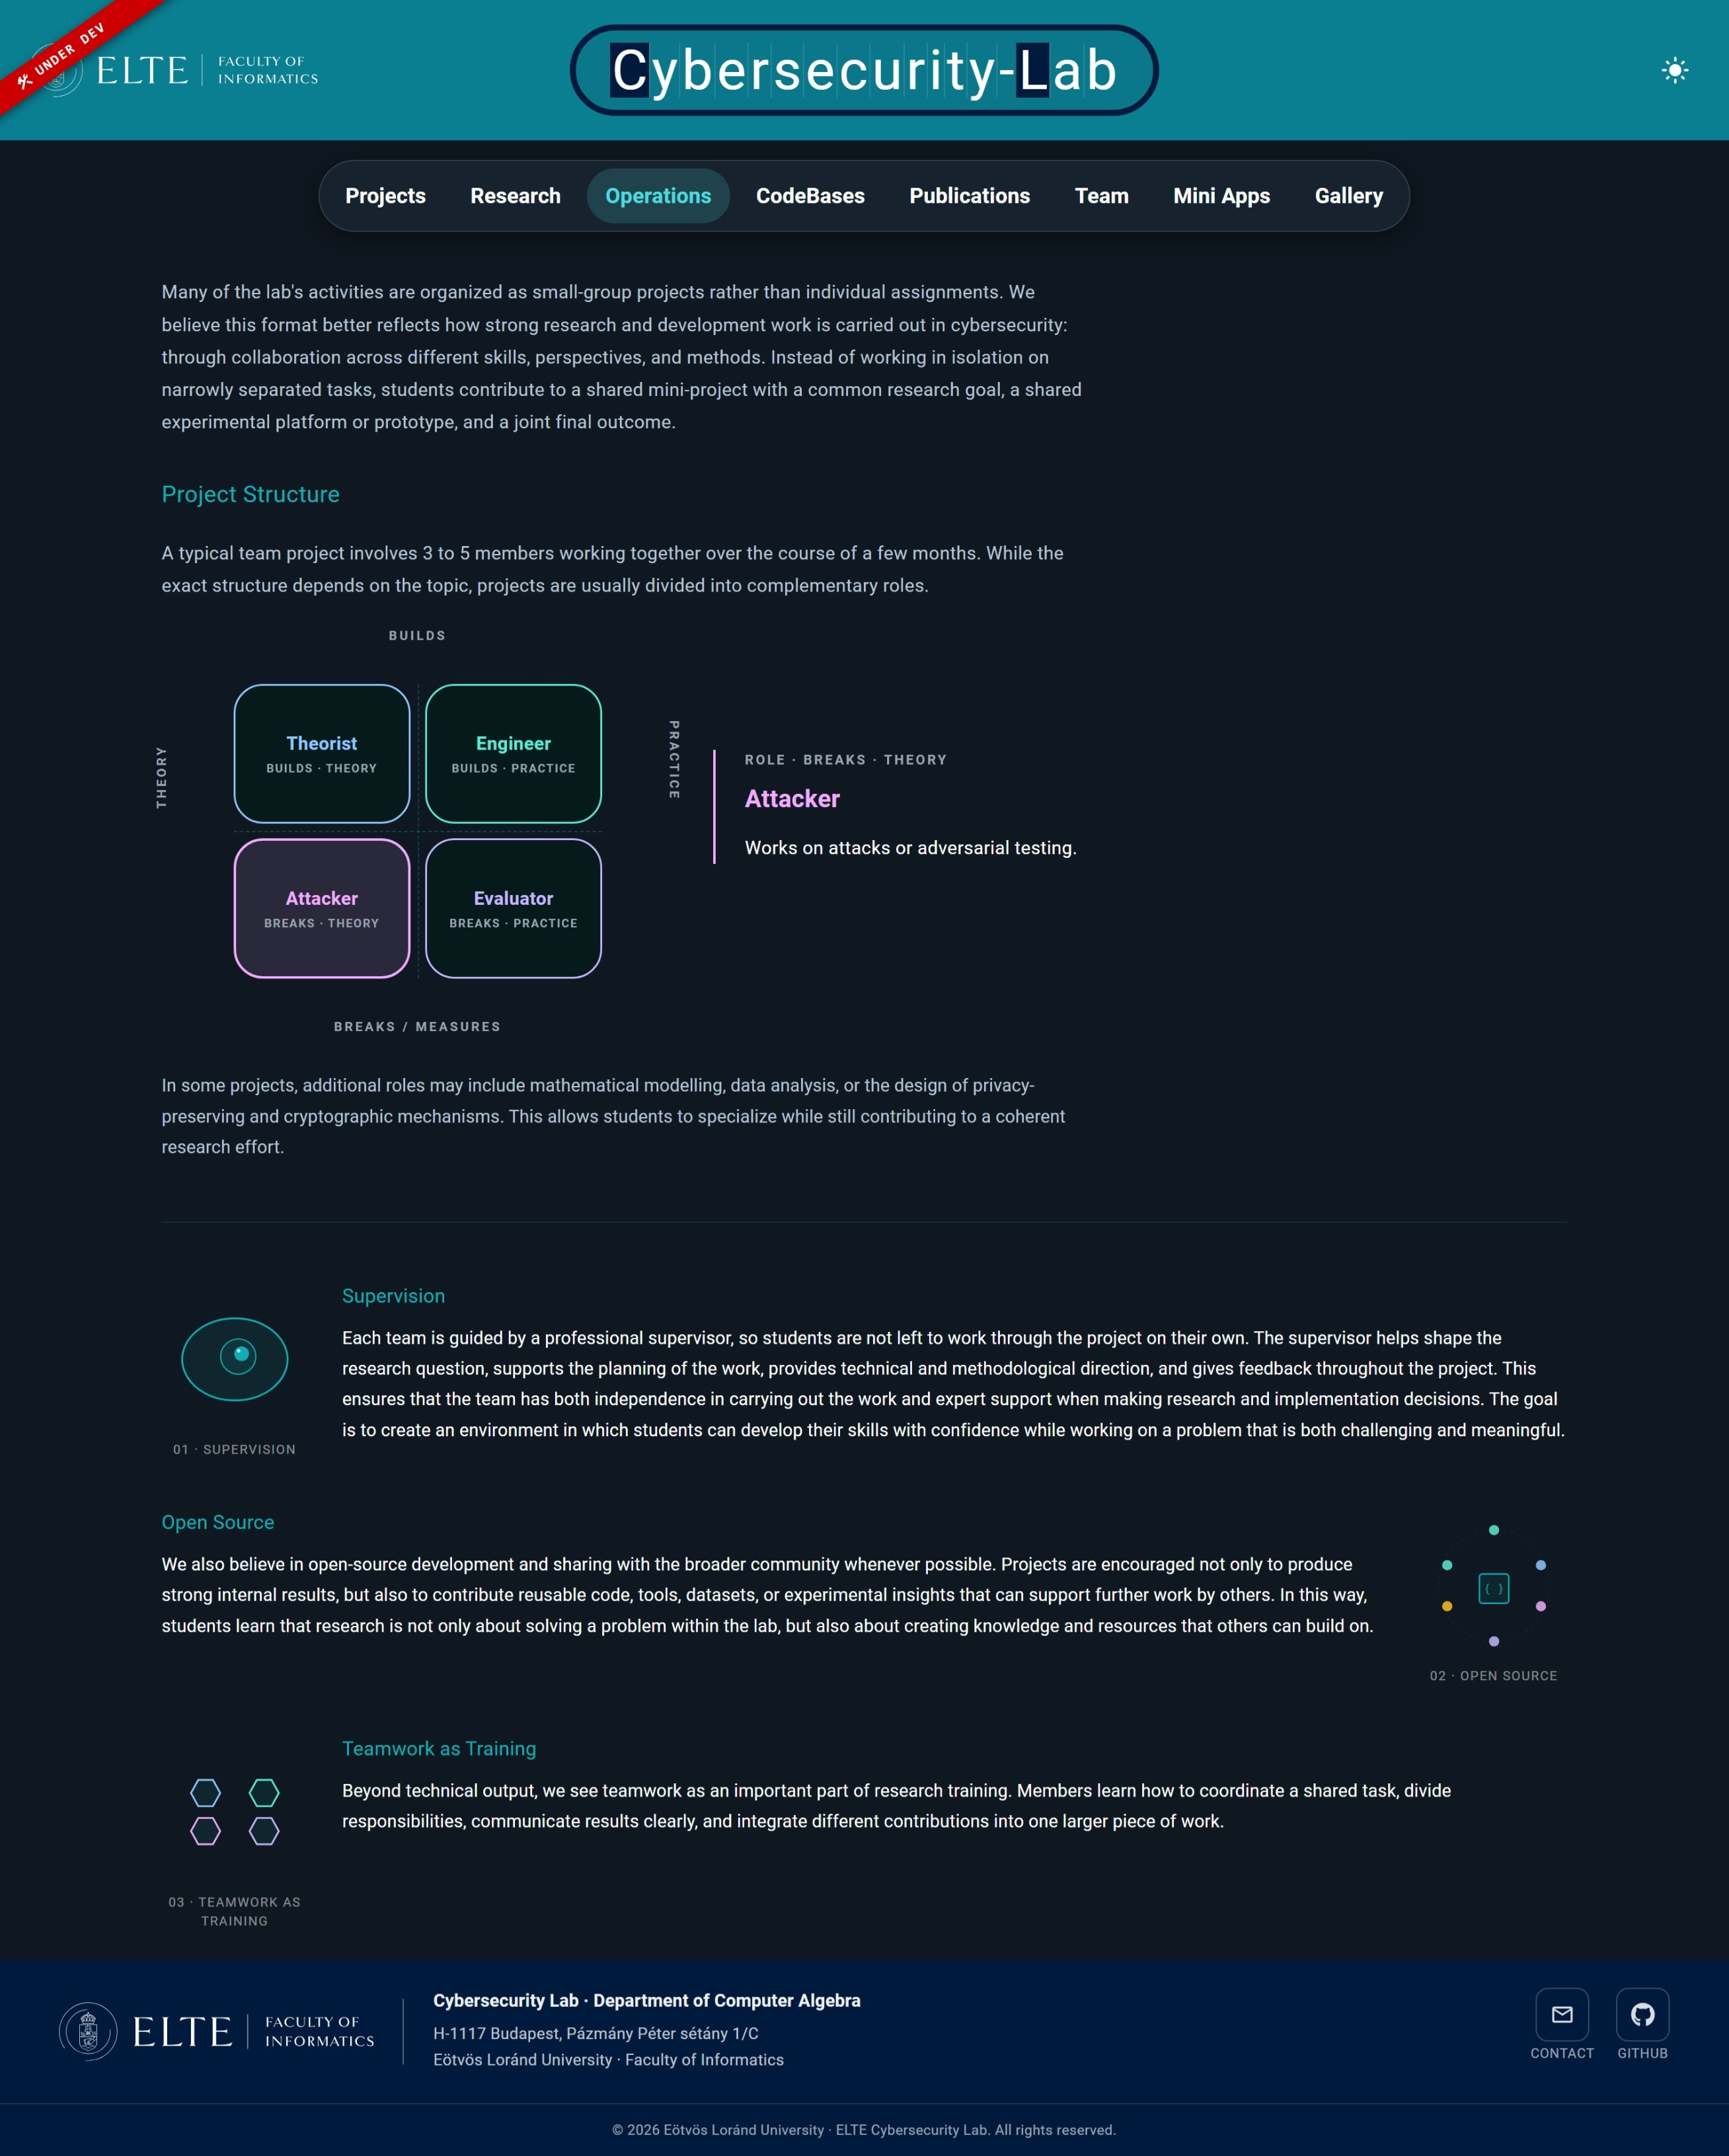
\includegraphics[width=0.88\textwidth]{images/operations.jpeg}
	\caption{The Operations page with the two-by-two role grid (the Attacker quadrant selected and showing its description on the right), and the three principles with their interactive visual components below.}
	\label{fig:operations-page}
\end{figure}

\paragraph{Data file.} The Operations page reads from \texttt{src/data/operationPageData.ts}. The file exports a single \texttt{operationPageData} object containing the intro paragraph, the structure heading and intro, the four roles (each with an \texttt{id}, \texttt{role}, \texttt{description}, axis assignment, and colours for both light and dark mode), the additional roles paragraph, and the three principles.

Each principle entry has an \texttt{id}, \texttt{title}, \texttt{description}, an optional \texttt{componentKey}, and an optional \texttt{iconFallback}. The \texttt{componentKey} field is what binds a principle to its interactive visual. The page keeps a small registry mapping component keys (\texttt{mentorEye}, \texttt{shareOrbit}, \texttt{teamPulse}) to the actual React components that render the visuals. When the page renders a principle, it looks up the \texttt{componentKey} in the registry; if the key is found, the corresponding visual is rendered, and if it is not found, the \texttt{iconFallback} value is used to render a Material UI icon instead. This means adding a new principle whose visual already exists in the registry requires no code changes at all; only a new entry in the data file. Adding a new visual requires adding one component file and one line in the registry, after which it is available to all data entries.

%-----------------------------------------------------------
\section{CodeBases Page}\label{sec:user-codebases}

The CodeBases page is the page the project was built around. It shows the lab's public repositories as a grid of cards, each card representing one repository. Each card shows the repository's logo (or a default icon if the repository does not have one), the repository's title, a short description, and two actions: \textbf{View repository} (which opens the GitHub page in a new tab) and \textbf{Open Project} (which opens the structured walkthrough for that repository).

Above the grid is a sort control with options for sorting by newest first, oldest first, title ascending, or title descending. The cards reorder on the page when the sort option is changed.

\begin{figure}[H]
	\centering
	
\includegraphics[width=0.88\textwidth]{images/codebases.jpeg}
	\caption{The CodeBases page with the grid of repository cards, each showing the project logo, title, short description, and two actions (View repository, Open Project).}
	\label{fig:codebases-page}
\end{figure}

Clicking \textbf{Open Project} loads a structured documentation view for the repository. On the left side of this view is a sidebar listing the topics of the documentation: \textbf{Overview}, \textbf{System Requirements}, \textbf{Hardware Setup}, \textbf{Software Installation}, \textbf{Build Instructions}, \textbf{Machines Overview}, \textbf{Configuration}, \textbf{Validation \& Testing}, \textbf{Troubleshooting}, and \textbf{References}. The exact list of topics depends on the repository; the sidebar is built from the structure of the Markdown document, not from a fixed list.

Clicking a topic in the sidebar loads only that topic into the main panel. The visitor reads one section at a time, in the same way they would read one chapter of a course at a time. At the bottom of each section there are \textbf{Back} and \textbf{Next} buttons that move to the previous and next topic in the sidebar. The current topic is highlighted in the sidebar and the highlight follows the visitor as they move through the documentation.

The content of each topic is rendered with full Markdown support: code blocks, tables, headings, links, lists, and images all render the way they would on GitHub. The lab's brand colour and dark theme are applied to the rendered content so the documentation looks like part of the portal rather than an embedded GitHub page.

\begin{figure}[H]
	\centering
	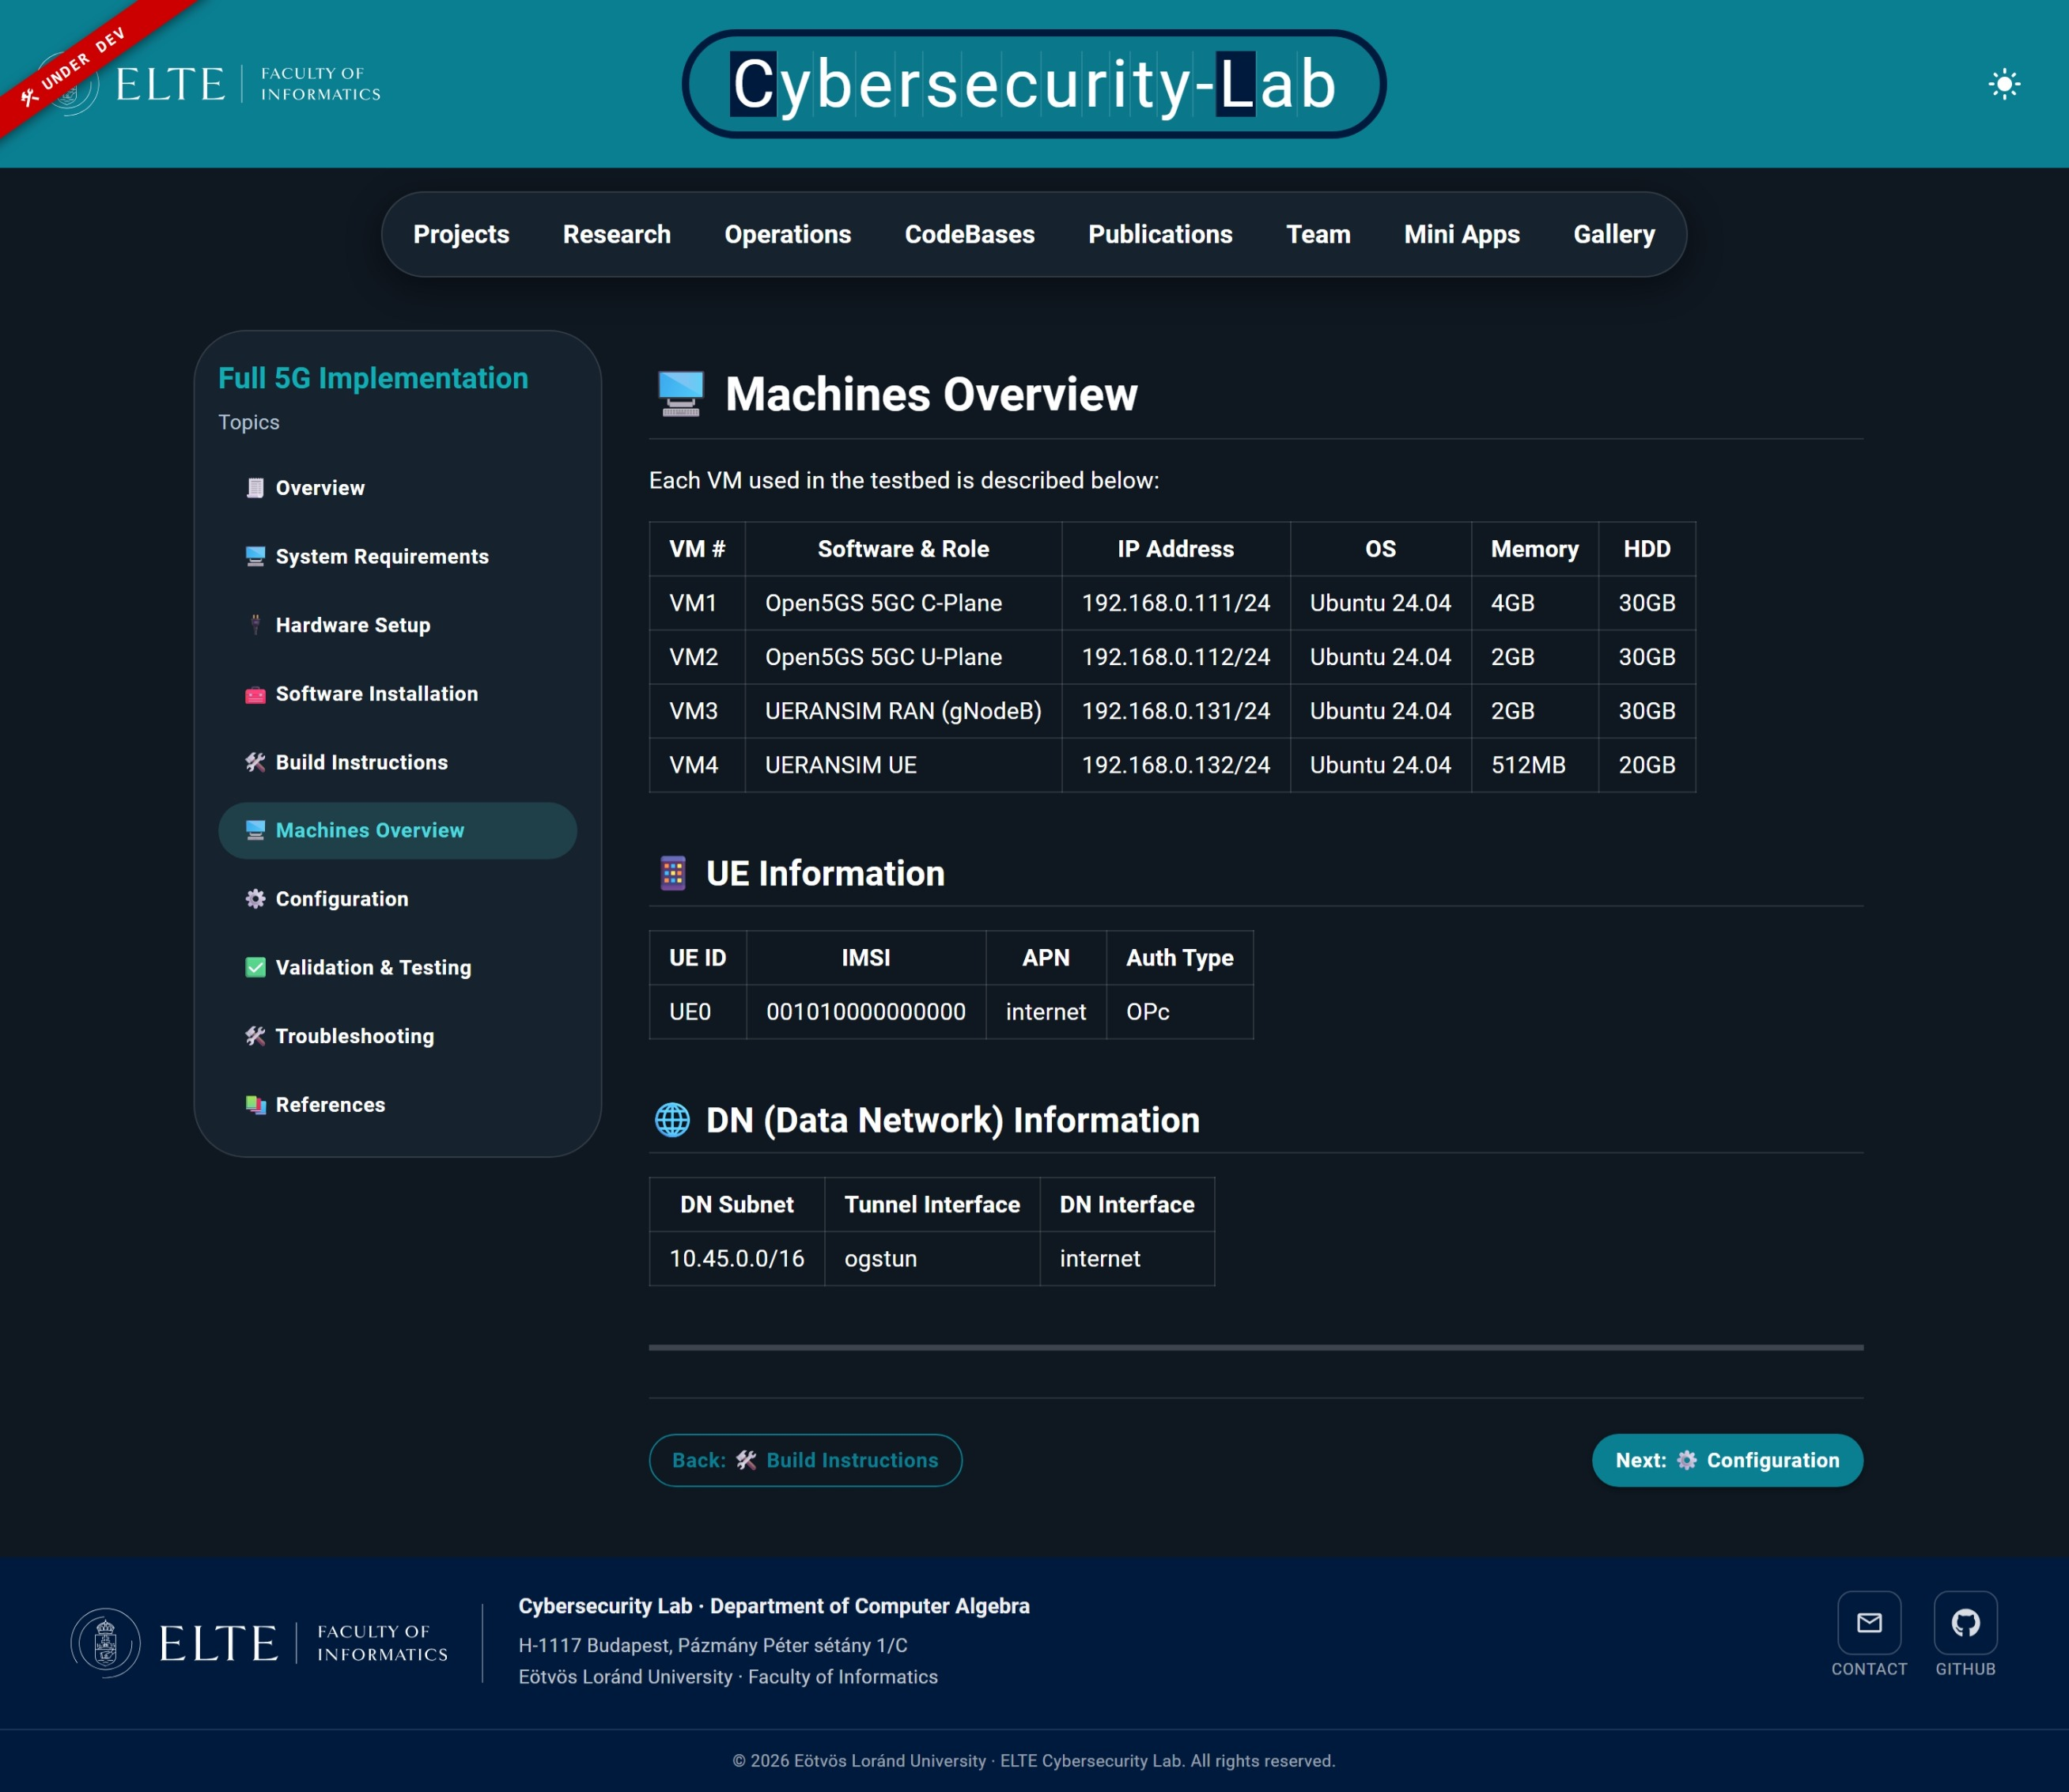
\includegraphics[width=0.88\textwidth]{images/codebase-sample.jpeg}
	\caption{A repository's detail view, showing the topic sidebar on the left and the rendered content of the selected topic (Machines Overview) on the right, with Back and Next buttons at the bottom.}
	\label{fig:codebases-detail}
\end{figure}

\paragraph{How the topics are decided.} The topics are taken directly from the Markdown file for the repository. The portal parses the file and uses the second-level Markdown headings (\texttt{\#\#}) as the top-level topics in the sidebar. Third-level headings (\texttt{\#\#\#}) become sub-topics inside a topic. The first-level heading (\texttt{\#}) is the repository's title. This is what makes the chapter-like feel work: the repository owner controls the structure of their own documentation by structuring the Markdown correctly, and the portal renders that structure as a navigable course.

\paragraph{Metadata block.} Each repository's Markdown file includes a small metadata block near the top, written as a \texttt{\#\# PORTAL\_METADATA} heading followed by a \texttt{portal} fenced code block. The block holds fields the portal uses to render the card on the CodeBases page: \texttt{slug}, \texttt{title}, \texttt{summary}, \texttt{startDate}, \texttt{endDate}, \texttt{repositoryUrl}, and a list of \texttt{logos}. The parser reads this block before walking the rest of the document and uses its values for the card and the routing. If the block is missing, the portal falls back to the file slug and a generic title.

\paragraph{Data file.} The list of repositories on the CodeBases page is built from the Markdown files in \texttt{src/content/}. Each file represents one repository's documentation and is loaded at build time by Vite. The metadata for each card (title, slug, summary, logos, etc.) comes from the metadata block inside each file, so adding a new repository to the portal is a matter of dropping a new \texttt{.md} file into \texttt{src/content/} that follows the agreed heading convention and has a valid metadata block. A template Markdown file is included in the project so anyone setting up a new repository for the lab can copy it and use it as a starting point.

%-----------------------------------------------------------
\section{Publications Page}\label{sec:user-publications}

The Publications page lists the lab's publications as a vertical list of rows. Each row shows the publication's ID, its type tag (\textbf{CONF} for conference, \textbf{JOUR} for journal, \textbf{BOOK} for book chapter), a small venue logo, the publication title, and the publication year. The row is collapsed by default and shows only this summary information.

Above the list is a filter section. There are four type filters at the top (\textbf{All}, \textbf{Conference}, \textbf{Journal}, \textbf{Book Chapter}) and three controls below: a search field that matches publication titles, a year input that filters by year, and an author dropdown populated automatically with the unique author names found in the publications data. Selecting a type filter or filling in any of the search controls narrows the list immediately.

Clicking a publication row expands it. The expanded view shows the authors, the venue with its logo, the abstract, a row of hashtag tags, and an \textbf{Access File} button. Clicking \textbf{Access File} opens the publication's URL in a new tab, where the visitor can find the full text.

The hashtags are clickable. Clicking a hashtag adds it to the active filter set as a removable pill, shown in a row labelled \textbf{ACTIVE} below the search controls. Multiple tags use AND semantics, so each additional tag narrows the list further. When two or more filters are active, a \textbf{Clear All} button appears next to them for one-click reset. Clicking a hashtag also automatically collapses the publication row and scrolls the page back up to the filter section so the visitor sees the new filter being added.

\begin{figure}[H]
	\centering
	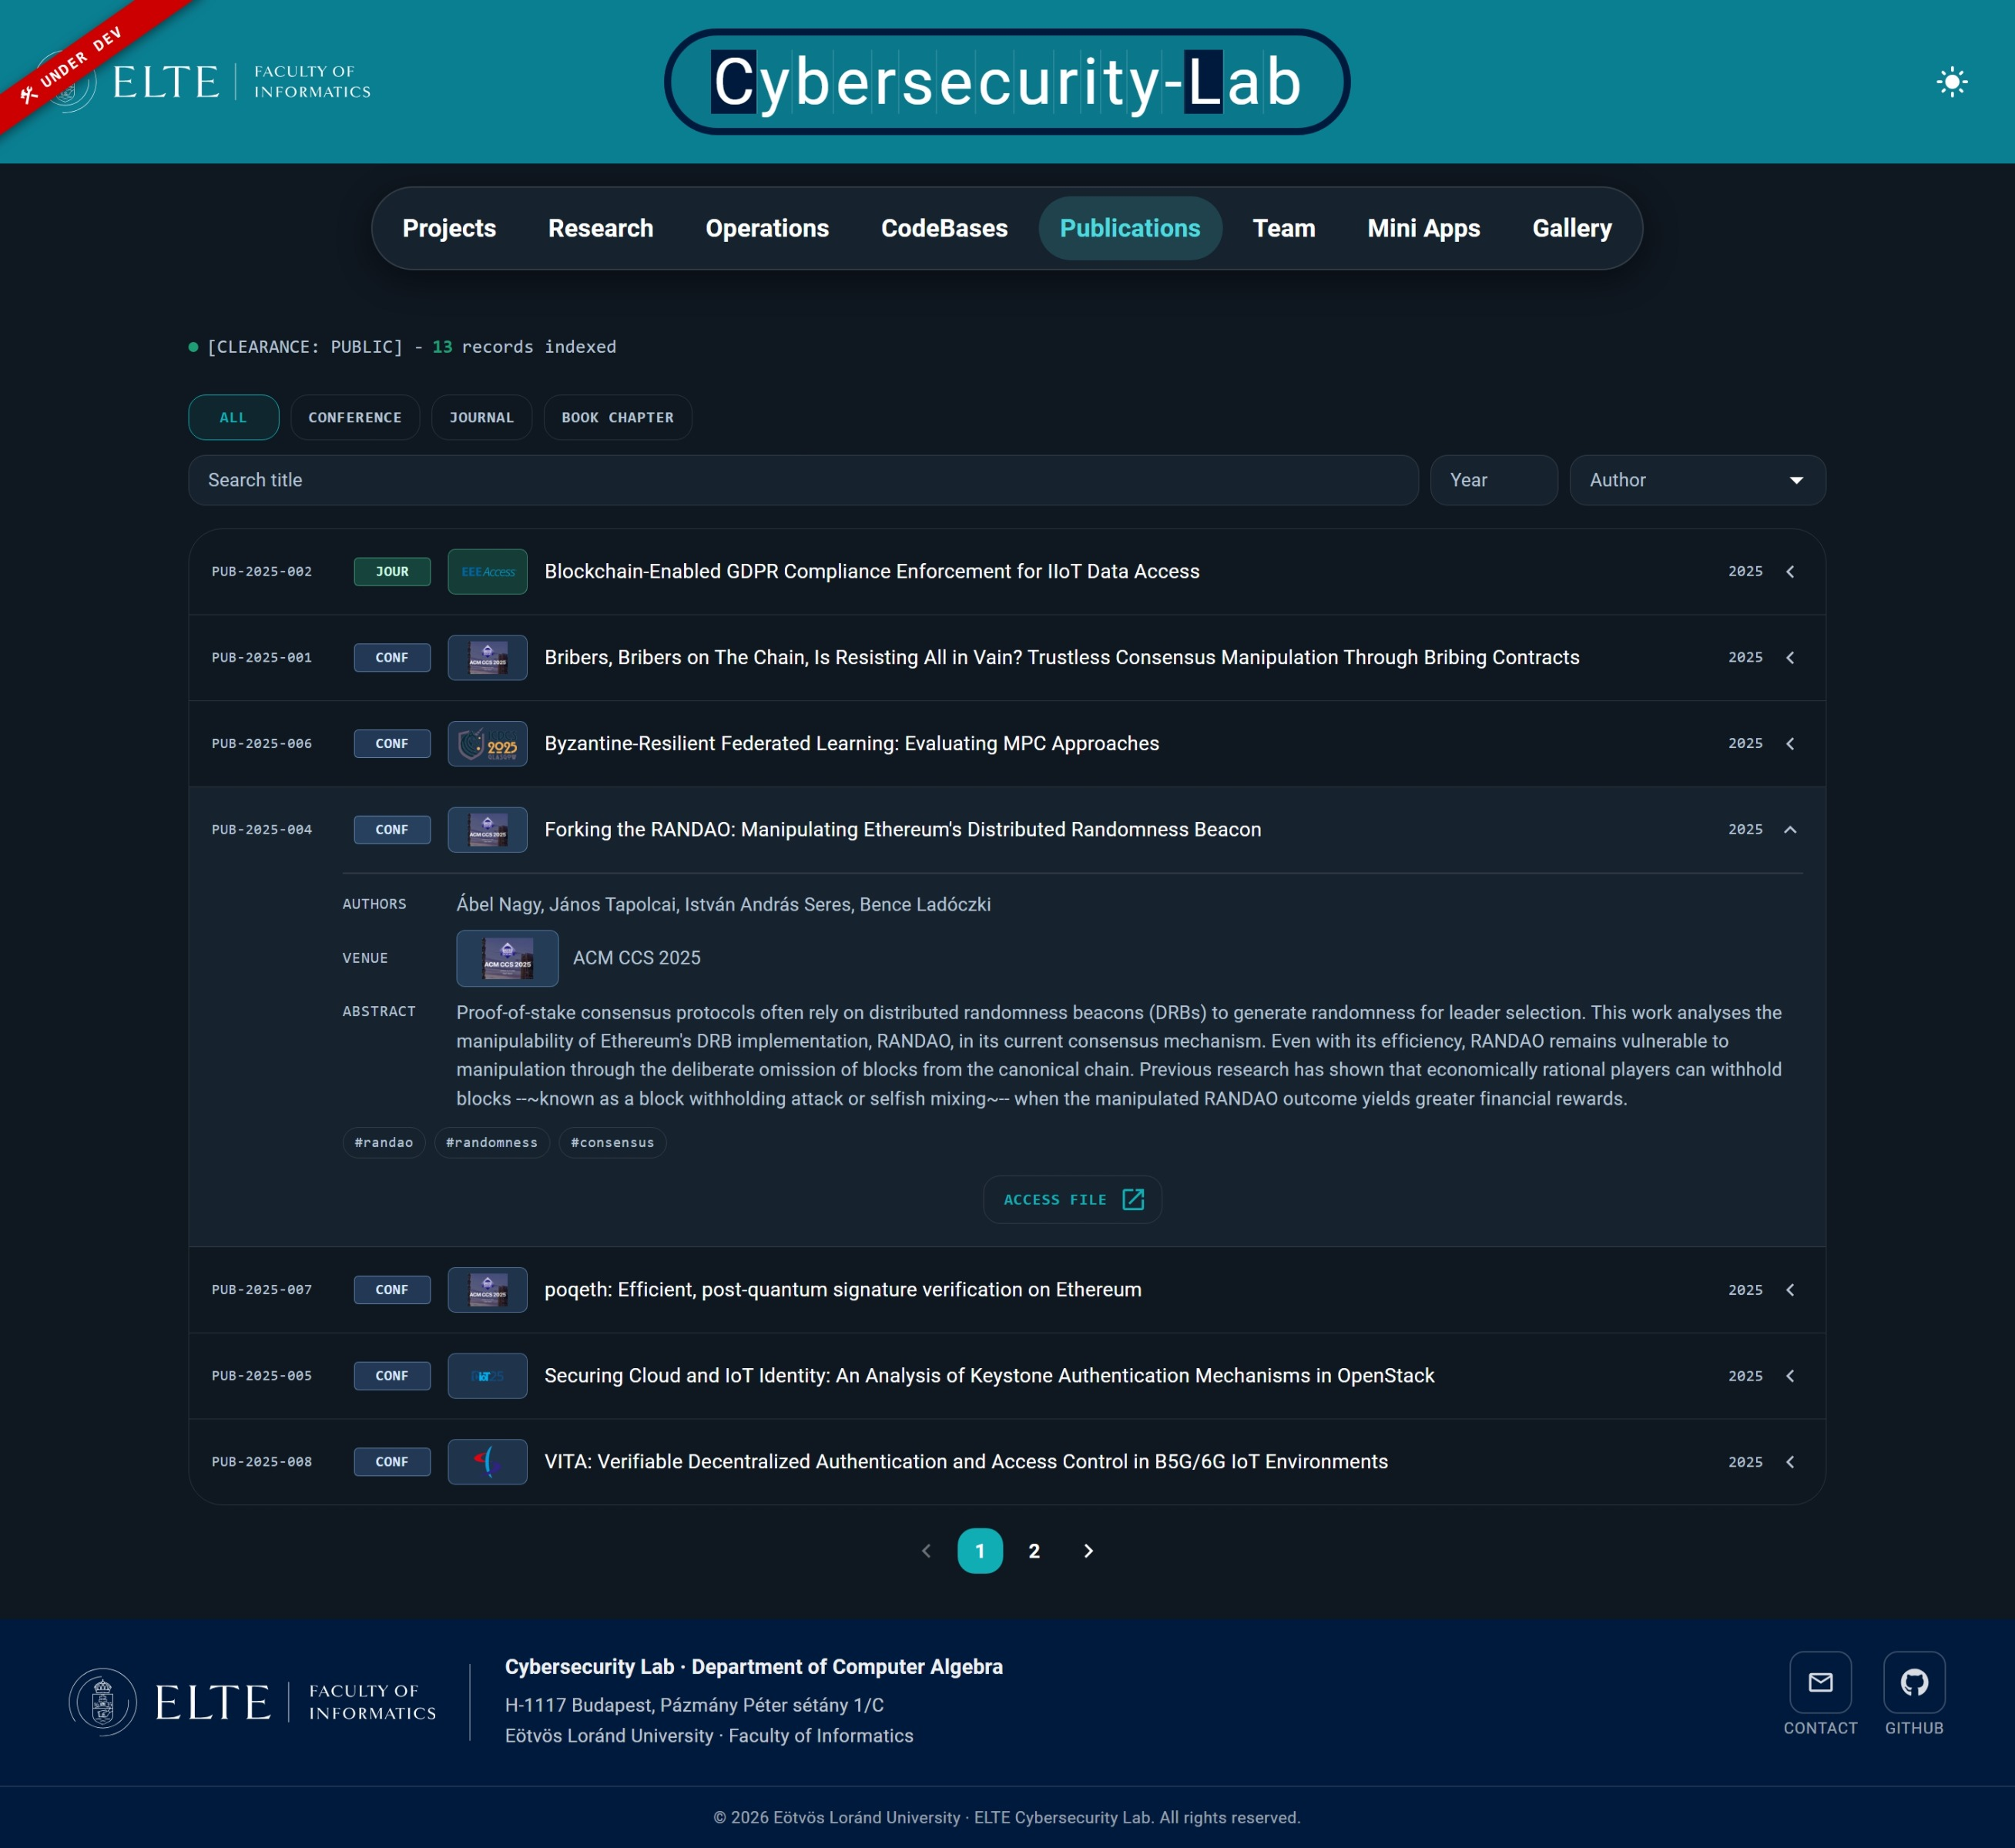
\includegraphics[width=0.88\textwidth]{images/publications_.jpeg}
	\caption{The Publications page with the type filters at the top, the search controls below them, and the publication list. The Forking the RANDAO entry is expanded to show its authors, venue, abstract, hashtags, and Access File button.}
	\label{fig:publications-page}
\end{figure}

\paragraph{Data file.} The Publications page reads from \texttt{src/data/publicationsData.ts}. Each publication entry has a code, a title, an author list, a venue, a year, a type (conference, journal, or book chapter), an abstract, a tag list, a URL pointing to the publication, and a \texttt{venueImage} field for the small logo shown next to the title. Adding a publication is a single new entry in this file. The type filters, the year input, the author dropdown, and the hashtag clicks all work off the same data with no other configuration needed.

%-----------------------------------------------------------
\section{Team Page}\label{sec:user-team}

The Team page introduces the people behind the lab. It is organised as a list of categories, each with its own group of members. The current categories are \textbf{Members} (the lab's faculty and researchers), \textbf{Developer} (the people who built the portal), and \textbf{Students Alumni} (former students of the lab).

Each category has a header row showing the category name, a thin divider, and the number of members in that category. The header is clickable and toggles the category open or closed. By default every category opens on first load.

Inside the \textbf{Members} and \textbf{Developer} categories, each member is shown as a full card: a circular avatar on the left (or a default avatar if no picture is provided), then the member's name (linked to their personal page if a link is set), their role, and a short biographical paragraph.

Inside the \textbf{Students Alumni} category, each member is shown as a smaller card containing just the avatar and the name. On desktop, alumni are paired two per row inside a shared bordered container with a vertical divider between the pair. On mobile, each alumnus is shown as its own card on its own row. The reason for two different layouts is a layout bug that appeared during development: the paired layout used a fixed grid that did not stack cleanly on mobile, and long alumni names like \textit{Arun Chittuparambil Polson} pushed the grid wider than the mobile viewport. The page now switches to single-card mobile layout below a certain breakpoint and the page no longer scrolls horizontally on small screens.

\begin{figure}[H]
	\centering
	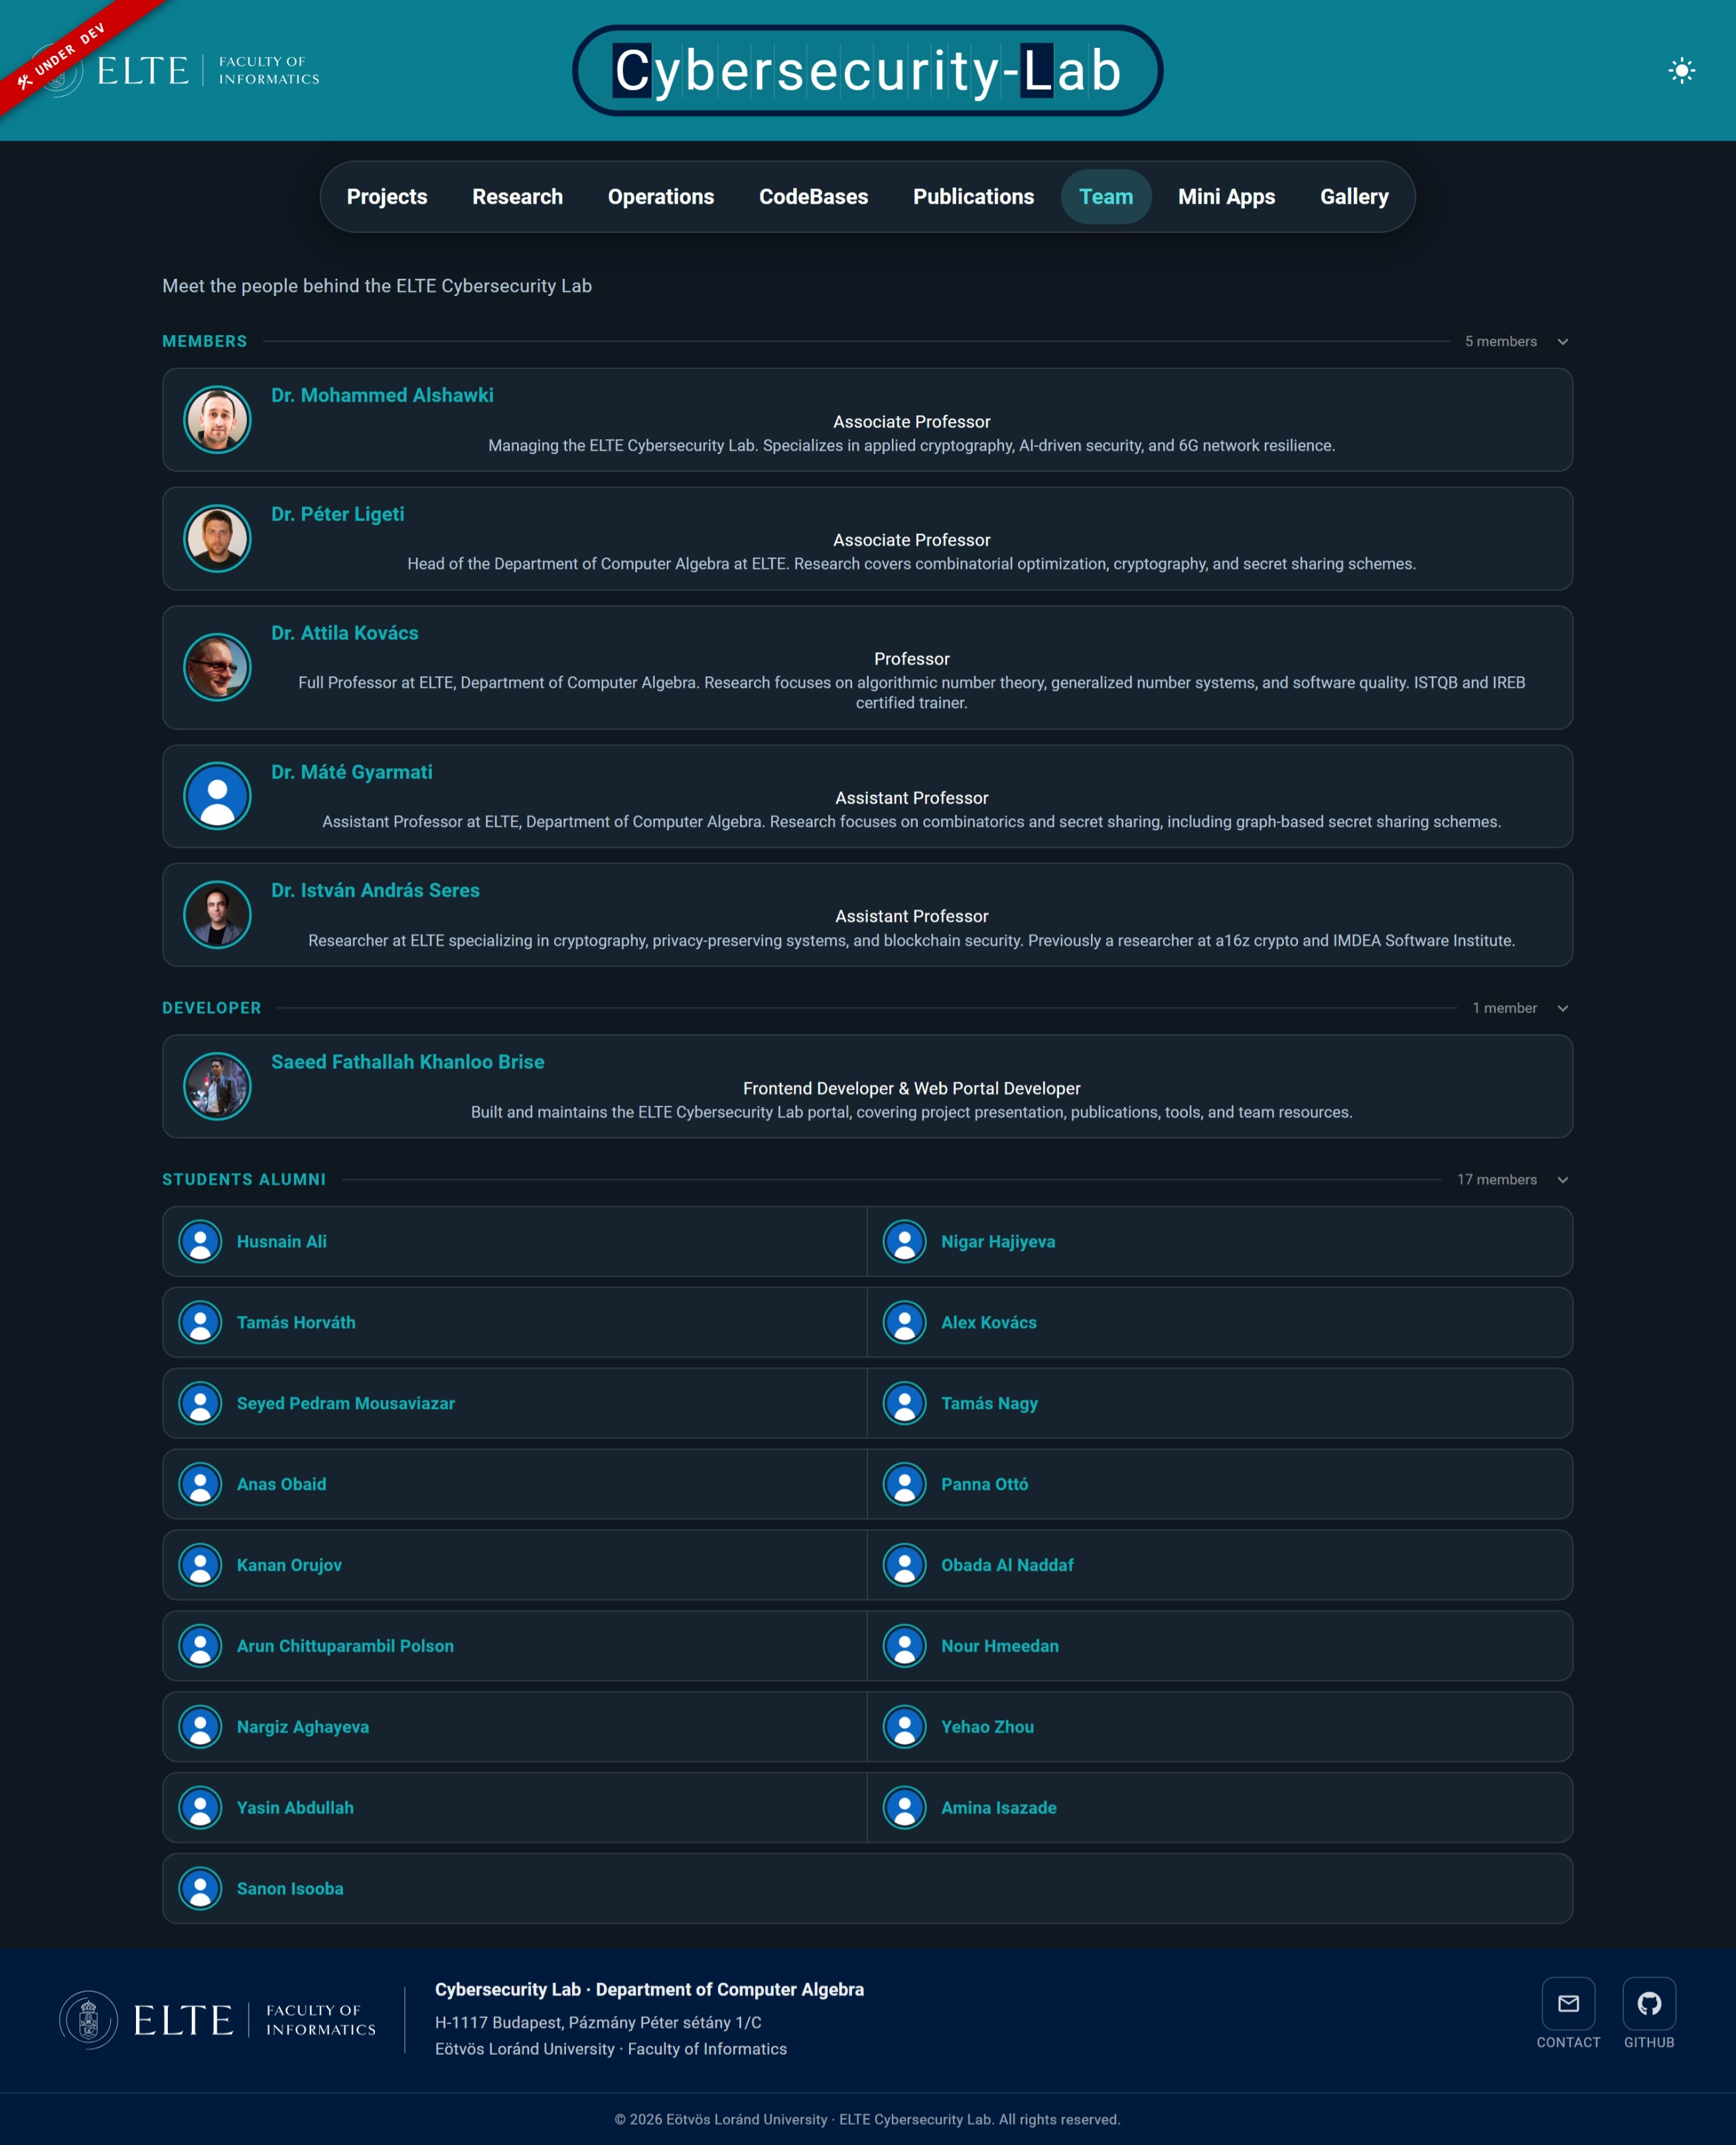
\includegraphics[width=0.88\textwidth]{images/team.jpeg}
	\caption{The Team page showing the Members, Developer, and Students Alumni categories. Members and Developer use the full card layout; alumni use the compact paired card layout on desktop.}
	\label{fig:team-page}
\end{figure}

\paragraph{Data file.} The Team page reads from \texttt{src/data/teamData.ts}. The file exports an array of \texttt{TeamCategory} objects, each with a \texttt{category} (the heading), and a \texttt{members} array. Each member has a \texttt{name}, \texttt{familyName}, \texttt{role}, \texttt{extraInfo}, \texttt{picture}, and \texttt{link}. The optional \texttt{title} field is for honorifics such as \textbf{Dr.} An empty \texttt{picture} field falls back to the default avatar. An empty \texttt{link} field renders the name as plain text instead of as a link.

The category order in the file is the category order on the page. Moving a member from one category to another is a matter of cutting and pasting the entry. Renaming a category renames its header. Adding a new category is a single new entry at the top level of the array.

%-----------------------------------------------------------
\section{Mini Apps Page}\label{sec:user-tools}

The Mini Apps page hosts the interactive tools and educational mini-applications built for the lab. At the time of writing there are two: \textbf{Ancient Cipher} and \textbf{Security Gauntlet}.

Each tool is shown as a card. The card has a square image at the top, two pill labels (a category label such as \textbf{Cryptography} or \textbf{Game}, and a status label such as \textbf{Live} or \textbf{Beta}), the tool's title, and a short description. Clicking the card opens the tool itself.

\textbf{Ancient Cipher} is a small encryption-and-decryption tool that supports classical ciphers (Caesar, Vigen{\`e}re). The visitor types in a message, picks a cipher, sets the cipher's parameters, and sees the encrypted or decrypted output update in real time. It is intended for teaching rather than for serious use; the goal is to give students an interactive way to play with the ciphers they read about in lectures.

\textbf{Security Gauntlet} is a collection of cybersecurity-themed mini-games, currently containing a Caesar cipher breakdown puzzle, a Keystone authentication packet-flow exchange, and a gradient defender game. The intent is for the gauntlet to grow over time as more games are added.

\begin{figure}[H]
	\centering
	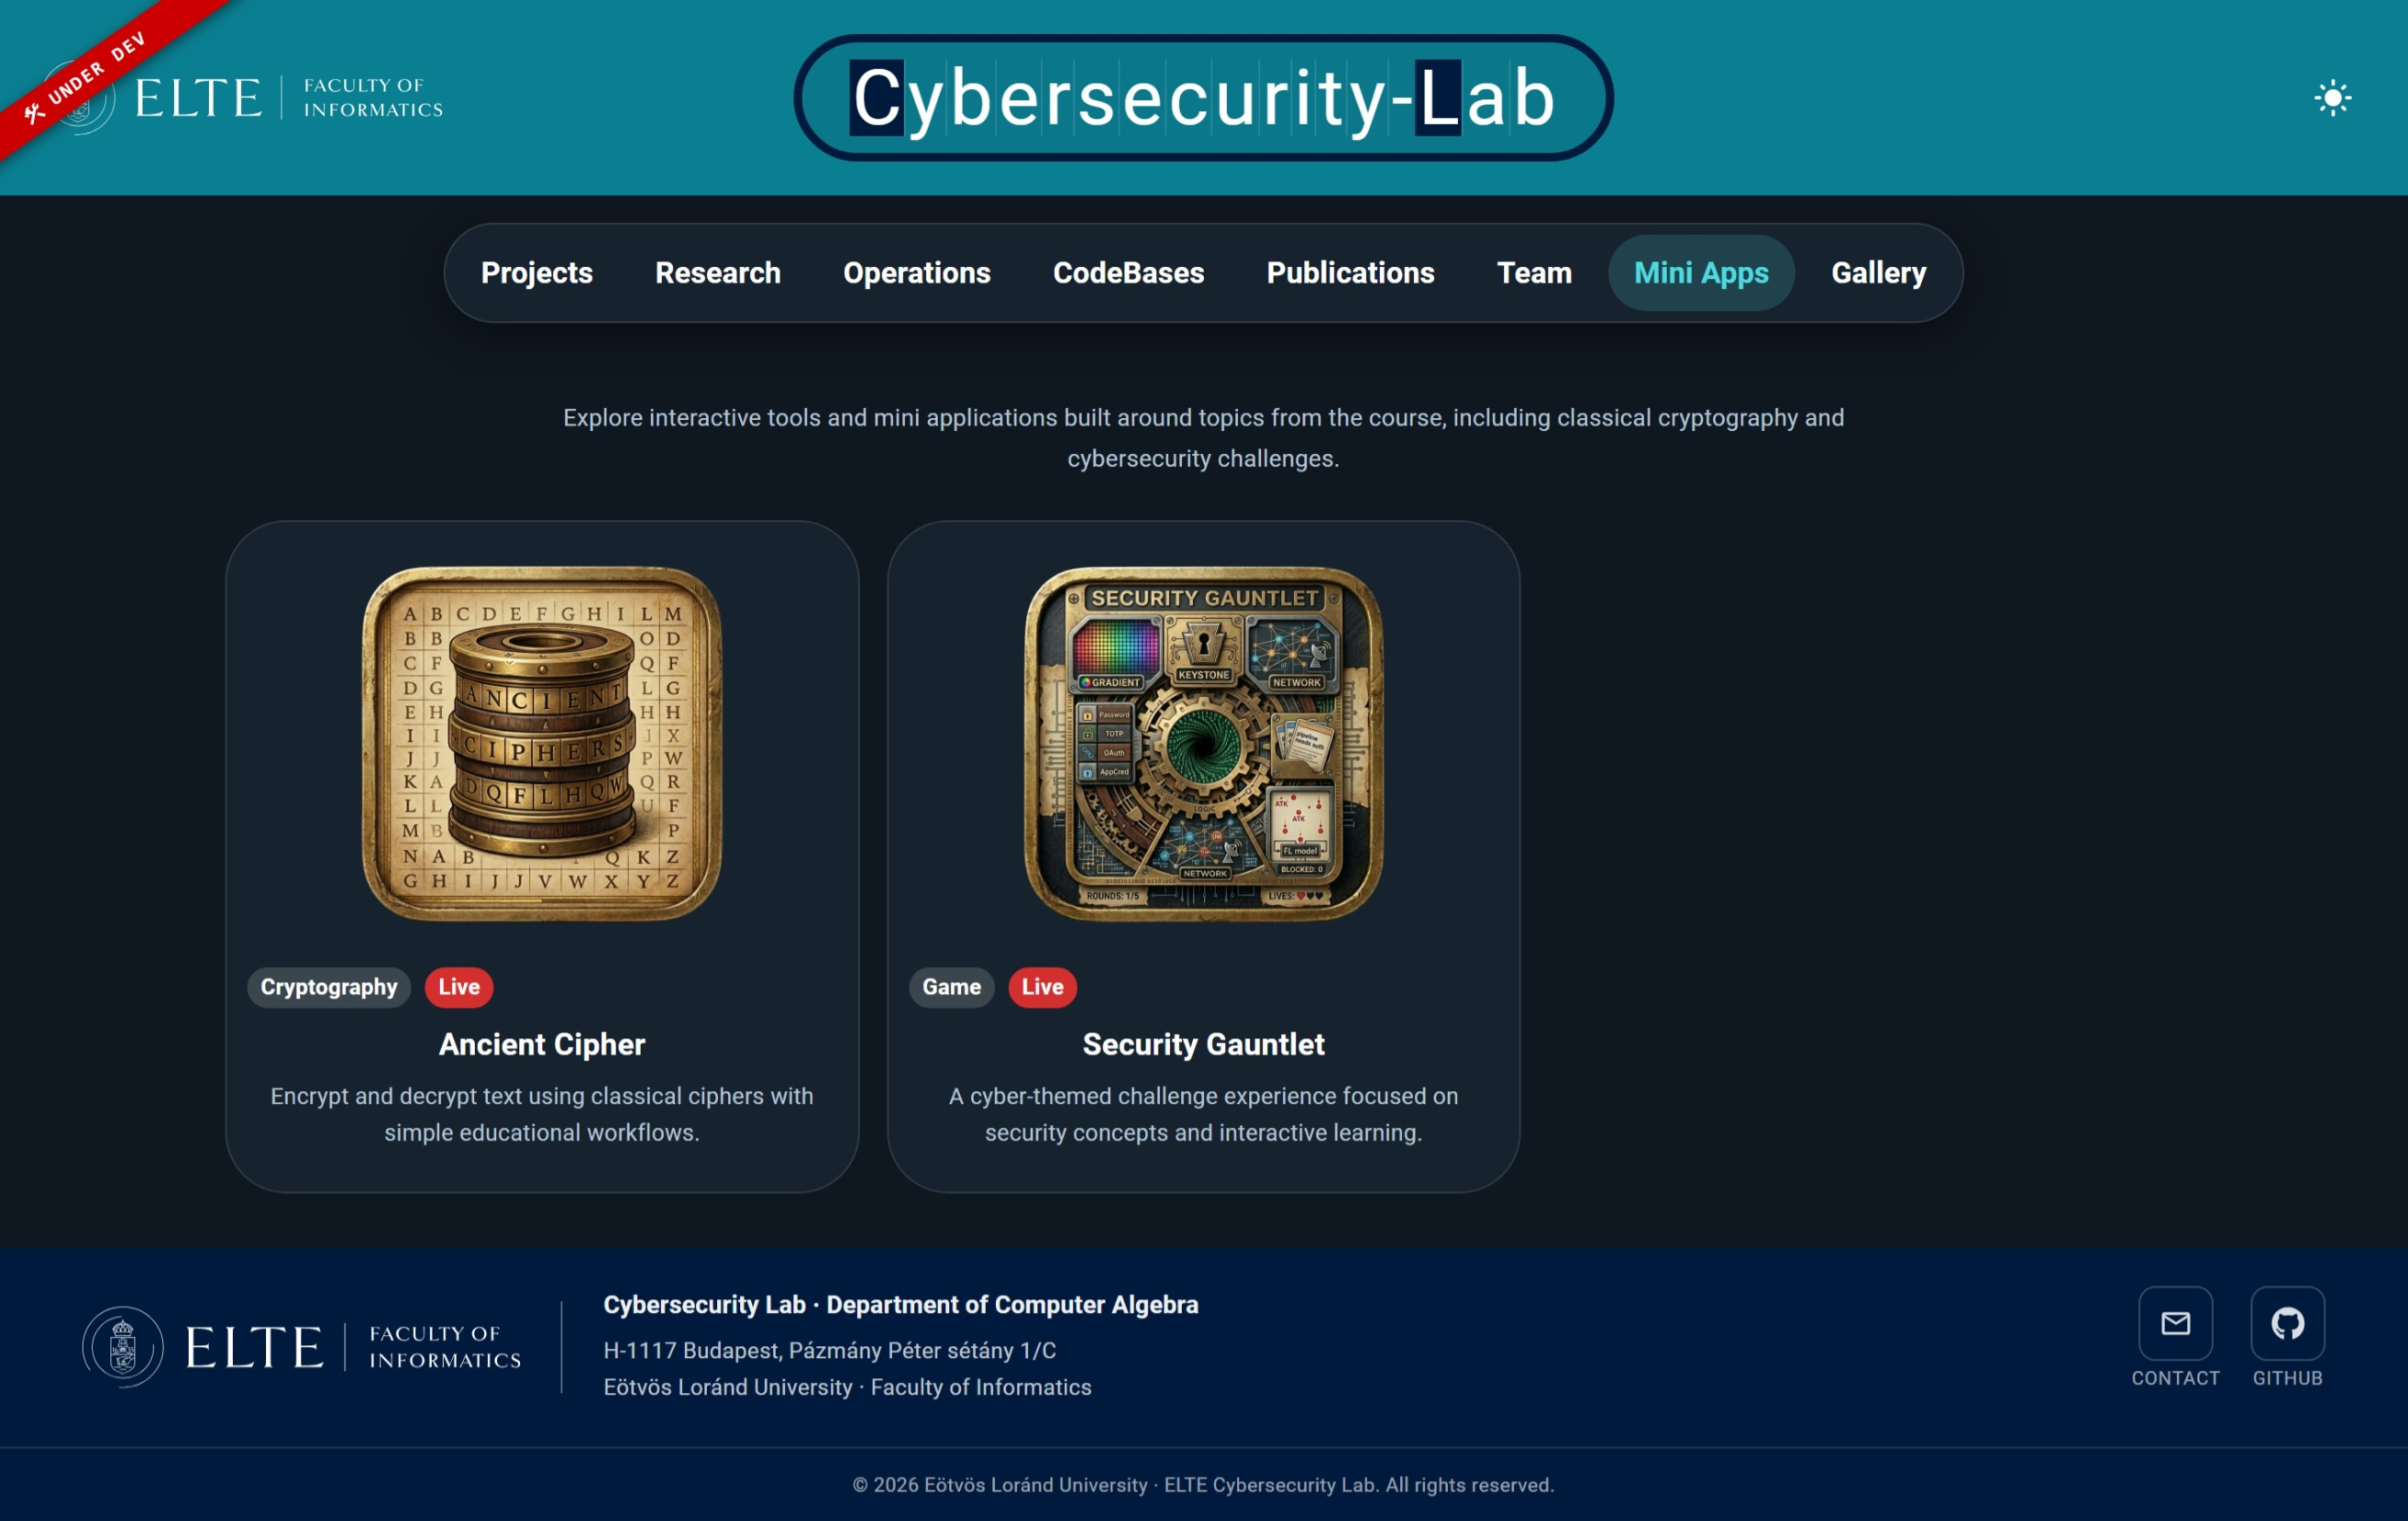
\includegraphics[width=0.78\textwidth]{images/mini-apps.jpeg}
	\caption{The Mini Apps page with two tool cards: Ancient Cipher (cryptography, live) and Security Gauntlet (game, live).}
	\label{fig:miniapps-page}
\end{figure}

\paragraph{Data file.} The Mini Apps page reads from \texttt{src/data/toolsData.ts}. Each tool entry has a \texttt{title}, \texttt{slug} (used as the route segment for the tool's page), \texttt{image} (a path to the card's image), \texttt{description}, optional \texttt{status} (\texttt{live}, \texttt{beta}, or \texttt{coming-soon}), and optional \texttt{category}. Adding a new tool requires the new entry in this file plus a route in the application that handles the tool's slug.

%-----------------------------------------------------------
\section{Gallery Page}\label{sec:user-gallery}

The Gallery page shows photographs of the lab, the university, and the campus. The photos are arranged onto stylised circuit-board-themed layouts, with three different board variants on desktop. The current layout shows the photo slot count at the top (e.g.\ \texttt{SECTION\_A // 04 SLOTS}) and arranges photos around drawn circuit traces with chip-like markers.

The visitor cycles through the available boards using the arrow controls on the sides of the layout. The pagination counter at the top of the page (e.g.\ \texttt{01 / 03}) shows the current board and the total. Clicking on any photo enlarges it for a closer look; clicking outside the enlarged photo collapses it back to the layout.

Three desktop board variants are available: a four-slot board (section A), and two three-slot boards (sections B and C). The portal picks a section for each page at random, with the constraint that the same section never appears twice in a row, so consecutive boards always use a different layout. If a section has more slots than the remaining photos provide, the empty slots are filled with the default photo so the board still looks complete. On mobile, the boards collapse to one photo per page to keep the layout readable on a narrow screen.

\begin{figure}[H]
	\centering
	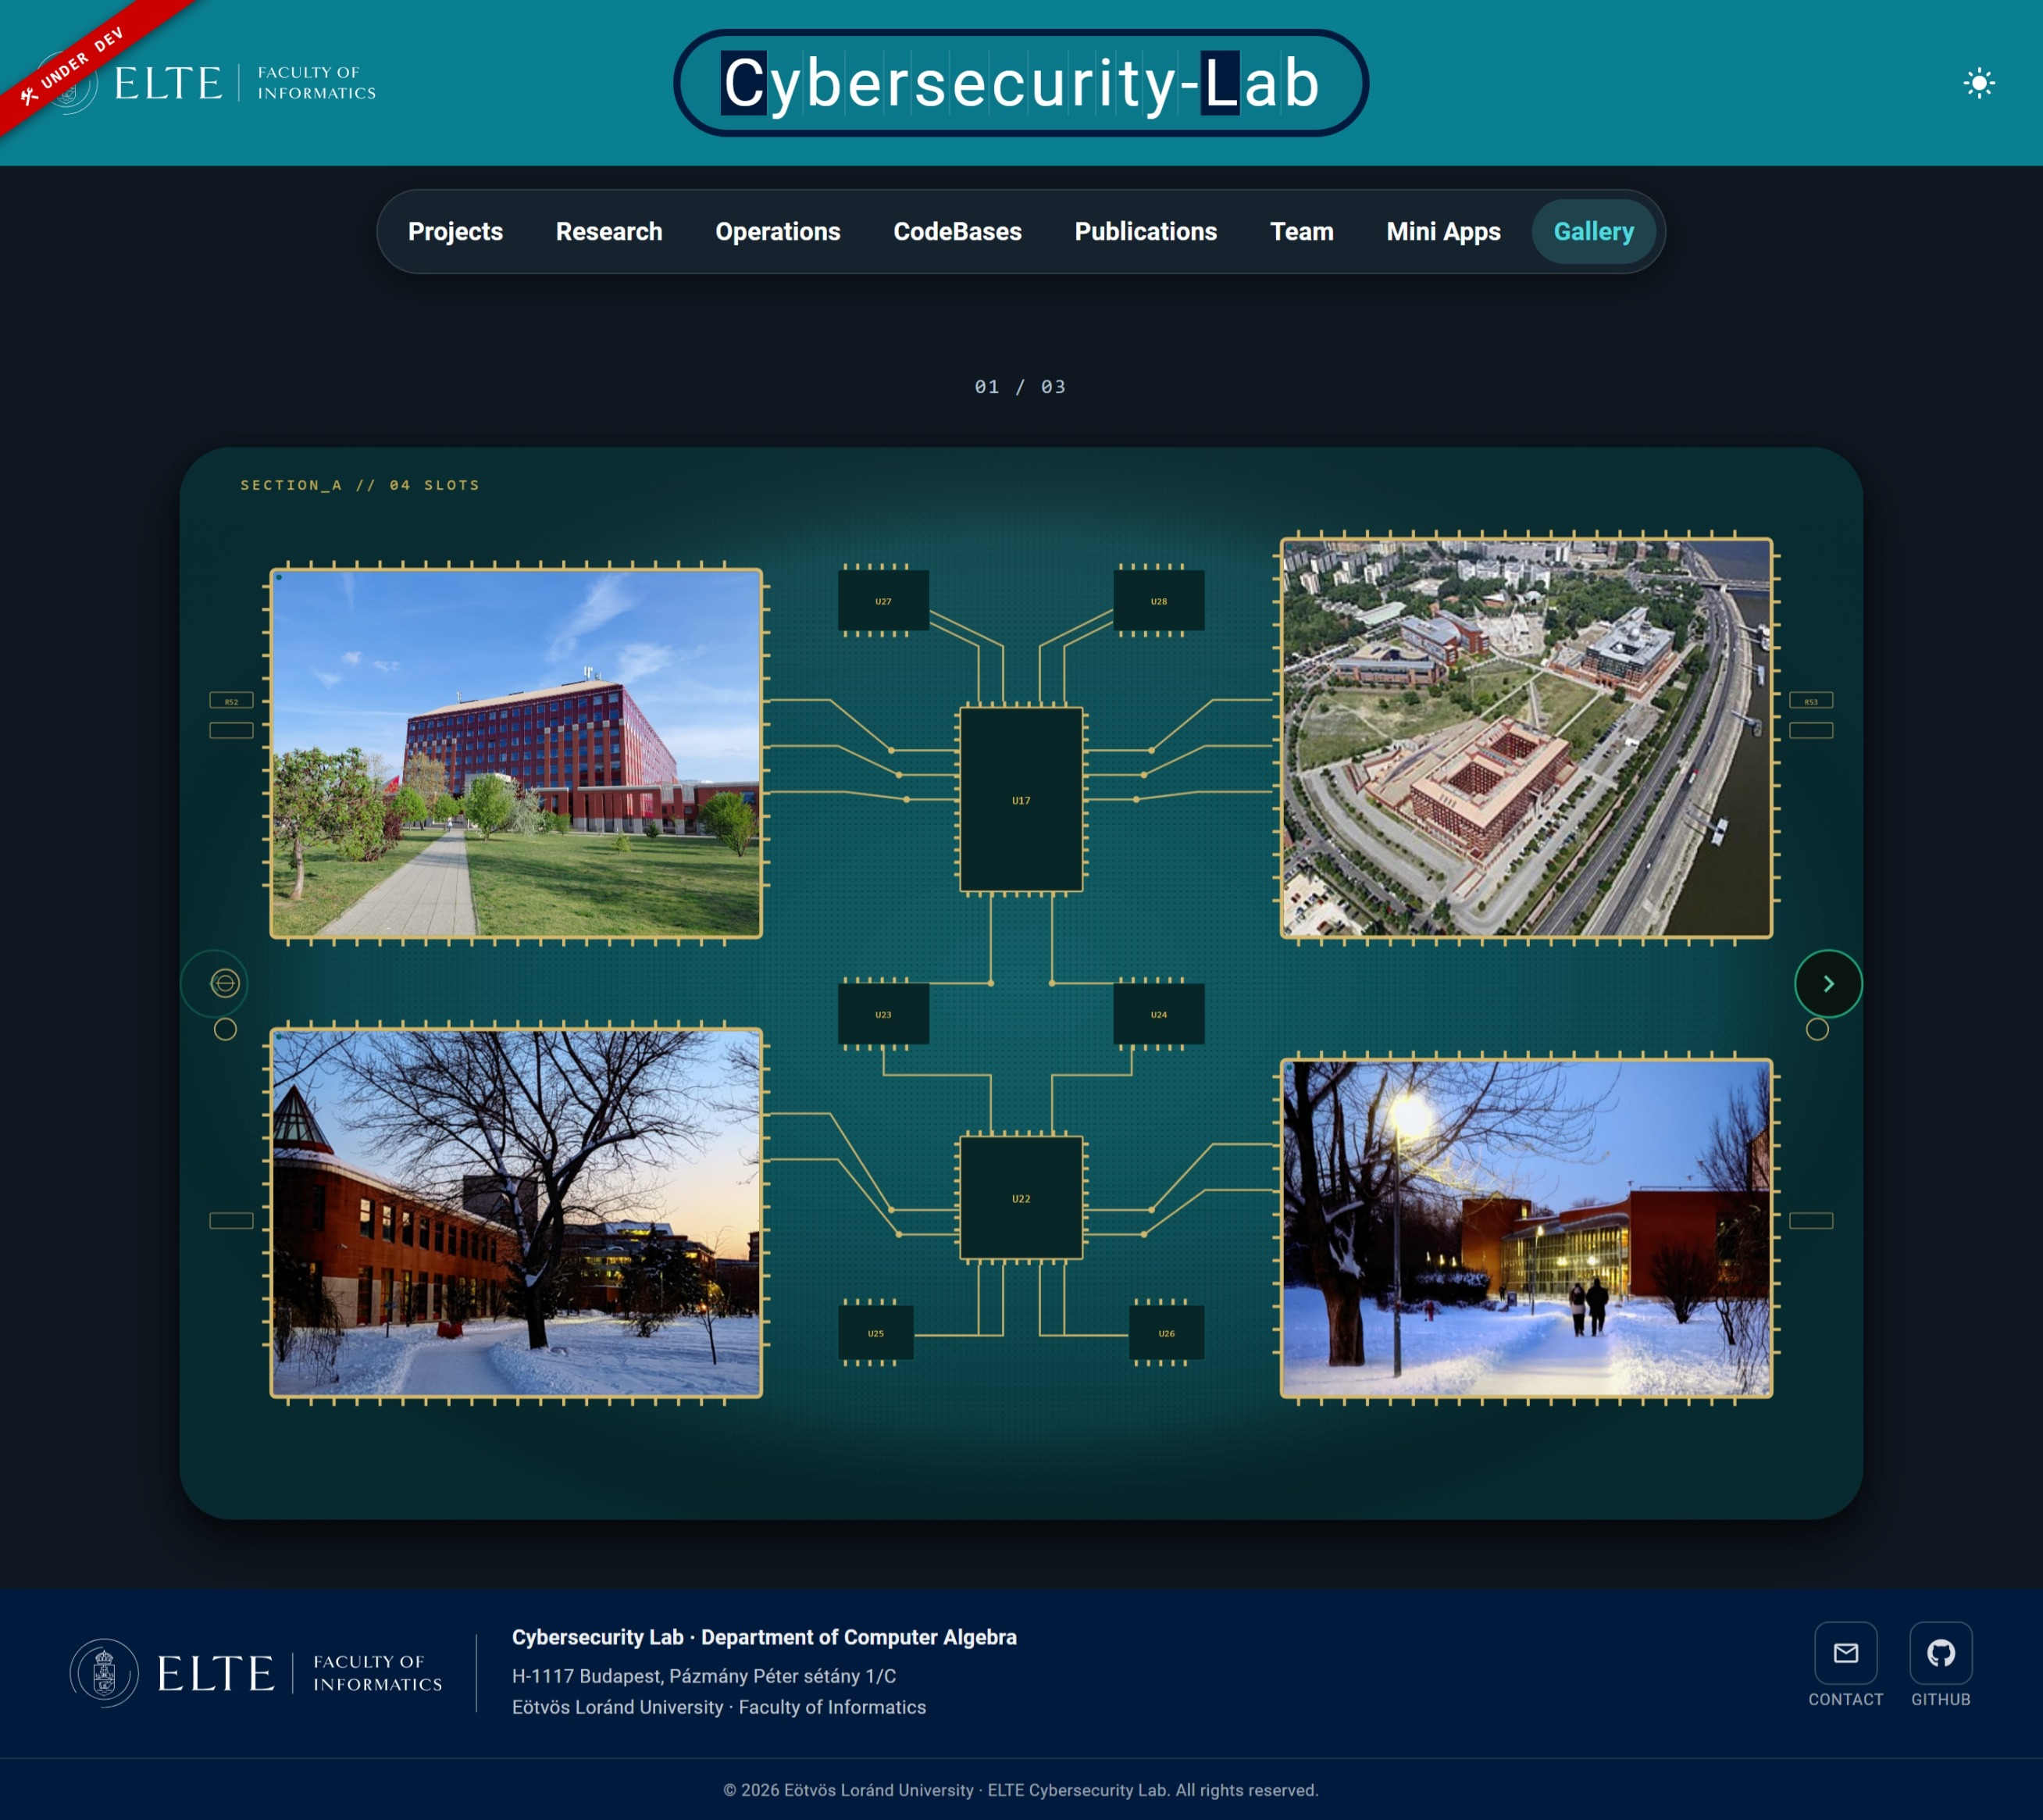
\includegraphics[width=0.88\textwidth]{images/gallery.jpeg}
	\caption{The Gallery page with a four-slot board (SECTION\_A) showing campus and lab photos arranged around drawn circuit traces. Arrow controls on the sides move to the next or previous board.}
	\label{fig:gallery-page}
\end{figure}

\paragraph{Data file.} The Gallery page reads from \texttt{src/data/galleryData.ts}. The file exports \texttt{galleryPhotos} (an array of file names), \texttt{defaultPhoto} (the file name used when a slot has no specific photo), and \texttt{galleryBasePath} (the directory where the photo files live in the \texttt{public/} folder). Adding photos is a matter of dropping the file into \texttt{public/gallery/} and adding its file name to the array. The portal handles the rest.

%-----------------------------------------------------------
\section{Contact Page}\label{sec:user-contact}

The Contact page is reachable from the \textbf{Contact} button in the footer rather than from the main navigation bar. It shows a single card titled \textbf{Contact} with a short paragraph (``Reach out for questions, collaboration, or general inquiries.''), an email line, and a phone line.

Below the contact details there is an \textbf{Open form} dropdown. Clicking it expands a contact form (name, email, message) inline below the contact card. The form is laid out but is not connected to a backend; submitting it does not currently send anything. The form is hidden behind the dropdown intentionally so that visitors who only want to copy the email or phone number do not have to scroll past an unused form.

The email and phone numbers shown on the page are currently placeholder values (\texttt{contact@example.com} and \texttt{+36 00 000 0000}). The lab is expected to replace these with the real values once they have decided what to publish.

\begin{figure}[H]
	\centering
	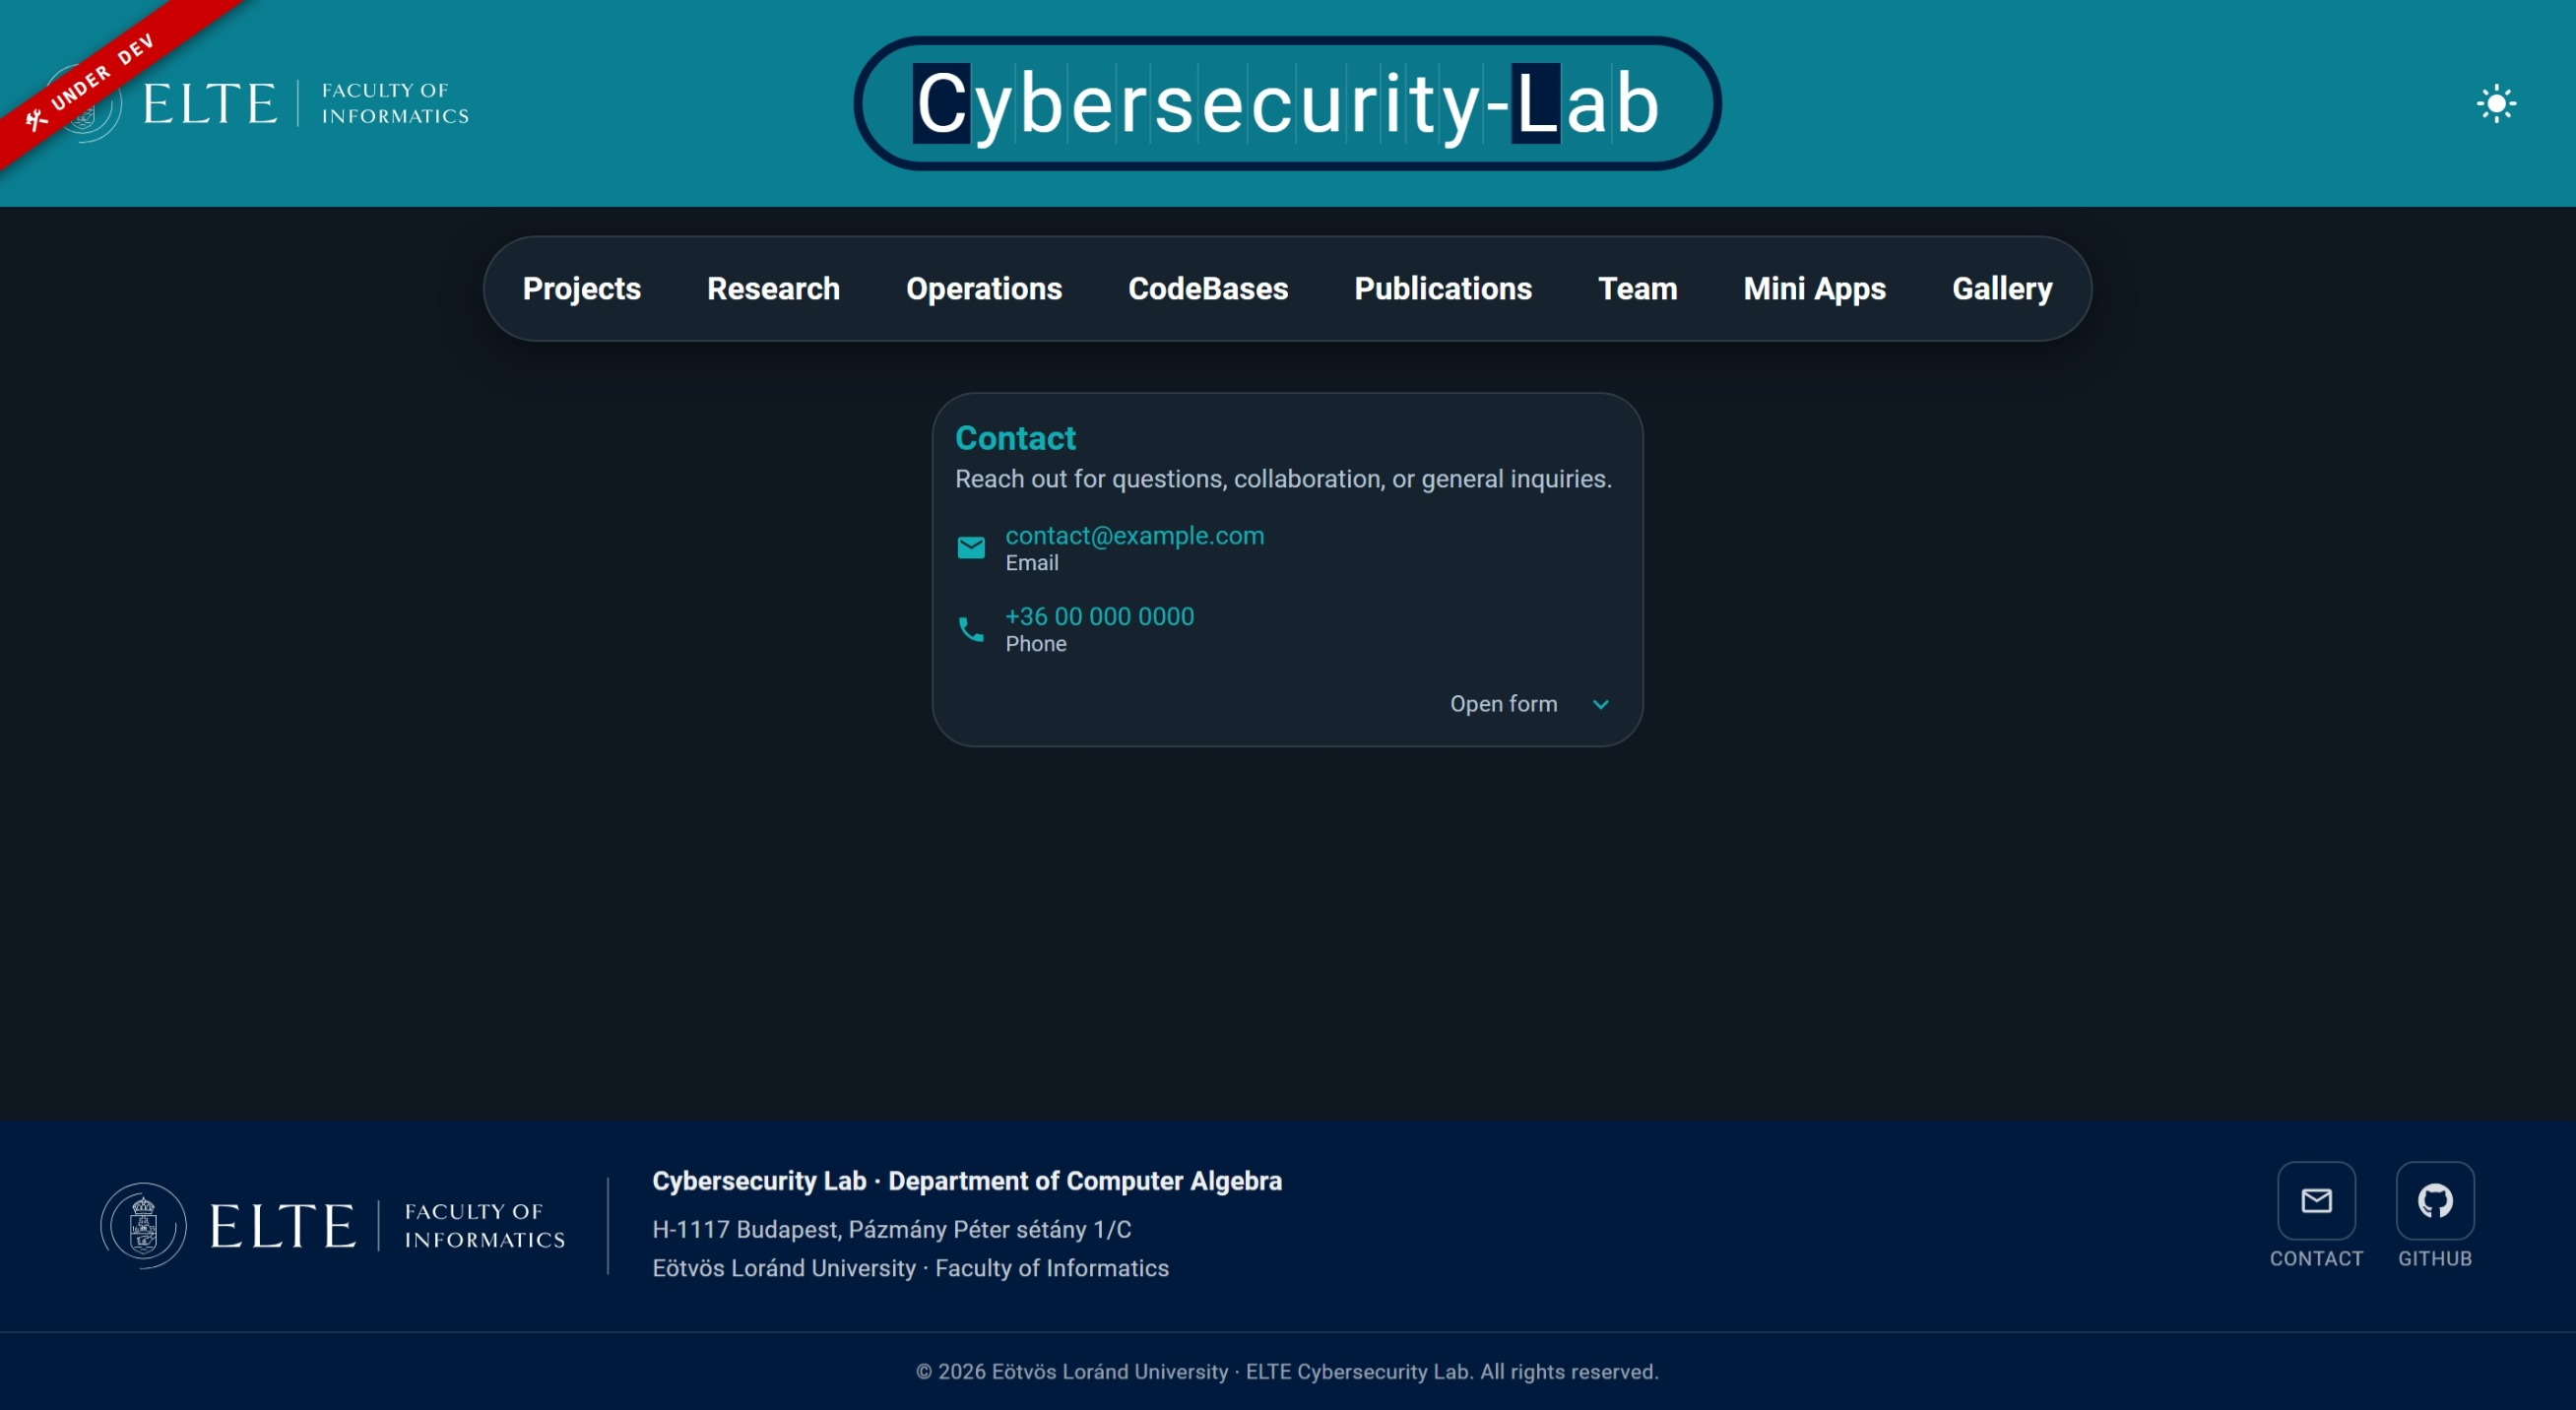
\includegraphics[width=0.88\textwidth]{images/contact-us.jpeg}
	\caption{The Contact page with the contact card showing the placeholder email and phone, and the Open form dropdown below for the contact form.}
	\label{fig:contact-page}
\end{figure}

\paragraph{Data file.} The Contact page reads from \texttt{src/data/contactPageData.ts}. The file is intentionally small: it has three fields, \texttt{email}, \texttt{phone}, and \texttt{showForm}. Setting \texttt{showForm} to \texttt{false} (the default) keeps the form behind the dropdown. Setting it to \texttt{true} would expand the form by default. The email and phone fields are plain strings.

%-----------------------------------------------------------
\section{GitHub Organisation Page}\label{sec:user-github}

The portal has a companion landing page on GitHub itself: the \texttt{profile/README.md} file in the \texttt{elte-cybersec/.github} repository, which GitHub renders as the organisation's profile page. This page is what visitors arriving through GitHub see first.

The GitHub organisation page mirrors the portal's structure rather than duplicating it. It has a waving banner at the top, an \textbf{About the lab} section, a \textbf{Research areas} grid with the same six areas as the Research page, a \textbf{Featured projects} grid with the lab's main public repositories, a \textbf{How we work} section that mirrors the Operations page, a \textbf{The team} section listing the lab manager and the scientific team, and \textbf{Get involved} and \textbf{Connect} sections that link back to the portal.

The intent is that visitors who arrive through GitHub do not have to leave GitHub to understand what the lab is about; they can read the organisation page and only follow the link to the portal if they want a more interactive experience. The two pages share the same brand colours and the same description text, so they feel like parts of the same identity. The top part of github page is shown in Figure~\ref{fig:github-org-page} on the next page.

\begin{figure}[H]
	\centering
	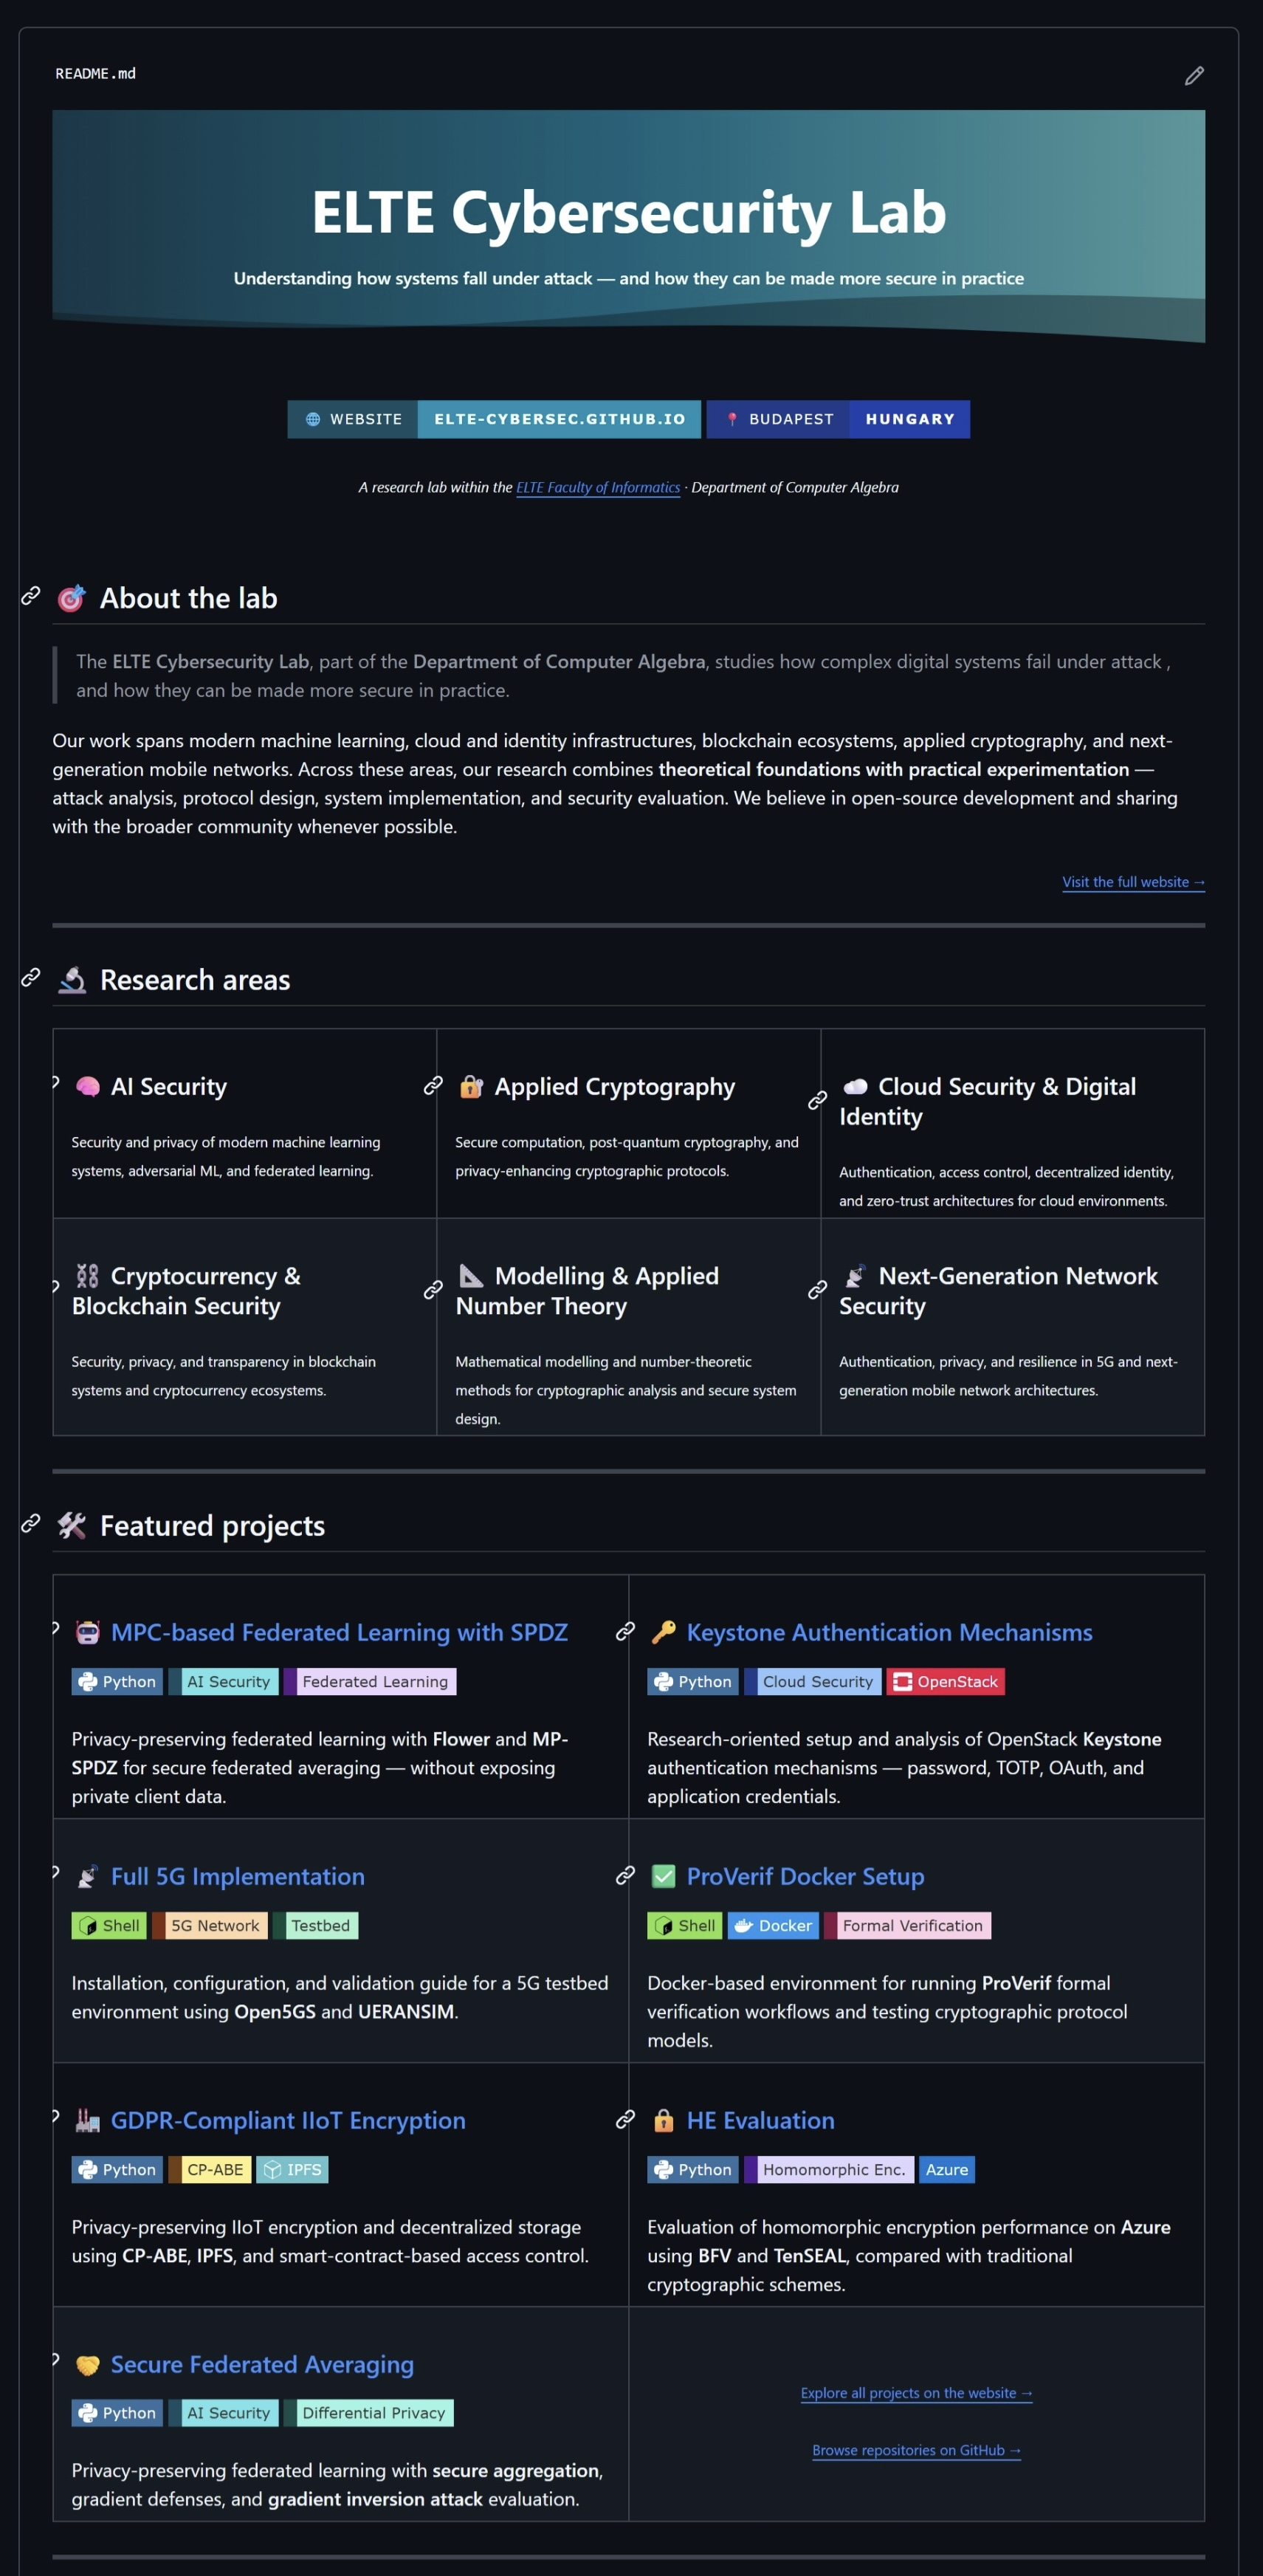
\includegraphics[width=0.75\textwidth]{images/github.jpeg}
	\caption{The ELTE Cybersecurity organisation page on GitHub, mirroring the structure of the portal with the about section, research areas, featured projects, how-we-work, team, and connect sections.}
	\label{fig:github-org-page}
\end{figure}